\documentclass[a4paper,11pt]{article}
\usepackage{ifpdf} 
\ifpdf
\pdfoutput=1 
\fi

\usepackage{jcappub}
\usepackage{graphicx}
\graphicspath{{Paper/}{./}}
\usepackage{dcolumn}
\usepackage{amssymb,amsmath,bm,bbold}
\usepackage{color}
\usepackage[dvipsnames]{xcolor}
\usepackage{xfrac}
\usepackage{aas_macros}
\usepackage{mathrsfs}
\usepackage{subcaption}
\usepackage{rotating}
\usepackage{chngcntr}
\newcommand{\nv}{\vec{\theta}}
\newcommand{\todo}[1]{{\bf TODO: #1}}

\newcommand{\as}[1]{{\textcolor{blue}{[AS: #1]}}}
\newcommand{\an}[1]{{\textcolor{magenta}{[AN: #1]}}}
\newcommand{\da}[1]{{\textcolor{red}{[DA: #1]}}}
\newcommand{\bh}[1]{{\textcolor{teal}{[BH: #1]}}}

\newcommand{\vd}{\mathbf{d}}
\newcommand{\vt}{\mathbf{t}}
\newcommand{\vN}{\mathbf{N}}

\newcommand\Tstrut{\rule{0pt}{3ex}}   

%\linenumbers

\definecolor{internationalkleinblue}{rgb}{0.0, 0.18, 0.65}
\hypersetup{urlcolor=internationalkleinblue, linkcolor=internationalkleinblue, citecolor=internationalkleinblue}

\usepackage[T1]{fontenc} % if needed
\usepackage{natbib}
\bibliographystyle{JHEP}
\title{Analytic marginalization of $N(z)$ uncertainties in tomographic galaxy surveys}

\author[a,1]{Boryana Hadzhiyska,}
\author[b]{David Alonso,}
\author[c]{Andrina Nicola,}
\author[d]{An\v{z}e Slosar}

\affiliation[a]{Harvard-Smithsonian Center for Astrophysics, 60 Garden St., Cambridge, MA 02138, USA}
\affiliation[b]{Department of Physics, University of Oxford, Denys Wilkinson Building, Keble Road, Oxford OX1 3RH, United Kingdom}
\affiliation[c]{Department of Astrophysical Sciences, Princeton University, Peyton Hall, Princeton NJ 08544-0010, USA}
\affiliation[d]{Brookhaven National Laboratory, Physics Department, Upton, NY 11973, USA}
\emailAdd{boryana.hadzhiyska@cfa.harvard.edu}

\abstract{We present a new method to marginalize over uncertainties in redshift distributions, $N(z)$, within tomographic cosmological analyses applicable to current and upcoming photometric galaxy surveys. We allow for arbitrary deviations from the best guess $N(z)$ governed by a general covariance matrix describing the uncertainty in our knowledge of redshift distributions. In principle, this is marginalization over hundreds or thousands of new parameters describing potential deviations as a function of redshift and tomographic bin. However, by linearly expanding the theory predictions around a fiducial model, this marginalization can be performed analytically, resulting in a modified data covariance matrix that effectively downweights the modes of the data vector that are more sensitive to redshift distribution variations. We showcase this method by applying it to the galaxy clustering measurements from the Hyper Suprime-Cam first data release. We demonstrate how we can marginalize over sample-variance of the PZ calibration sample and a large general systematic uncertainty in photometric determination methods, and explore the impact of priors imposing smoothness in the redshift distributions. We find that this method gives results that are comparable to the ad-hoc shift and width parameterizations, and discuss the applicability of the method to ``3$\times$2-point'' analyses and future surveys (and show that the only deviations that matter are smooth deviations \da{are we really doing this?}). 
}


\begin{document}
\maketitle
\flushbottom

  \section{Introduction}\label{sec:intro}
    Photometric galaxy surveys  have the potential to transform our understanding of the Universe by measuring the properties of millions and soon billions of galaxies on the sky. These catalogs can be used to constrain cosmological parameters from measurements of galaxy clustering and weak gravitational lensing as demonstrated by numerous surveys, including the Sloan Digital Sky Survey \cite{astro-ph/0006396,2013MNRAS.432.1544M}, PanSTARRS \cite{2010SPIE.7733E..0EK}, Kilo-degree Survey \cite{1206.1254,2020A&A...633A..69H}, Dark Energy Survey \cite{1601.00329,2018PhRvD..98d3526A}, Hyper Suprime-Cam survey (HSC) \cite{2012SPIE.8446E..0ZM,2019PASJ...71...43H,1912.08209}, and will play a crucial role in the upcoming Vera Rubin Observatory Legacy Survey of Space and Time \cite{0912.0201}.

    It has been long recognized that the constraining power of photometric surveys relies heavily on the accuracy of photometric redshift distributions and that this is likely to continue to be a dominant source of systematic uncertainty. The crucial quantity is the redshift distribution $N(z)$, which is simply the mean number of galaxies as a function of redshift for each tomographic sample. It is known that the accuracy in the shape of $N(z)$ delivered by the current photometric redshift codes and subsequent calibrations is insufficient for retiring this source of systematic error completely \cite{1809.01669}. Improving photometric redshift techniques and calibration methods for redshift distributions is an area of active research \cite{2006A&A...457..841I,2008ApJ...684...88N,2012MNRAS.423..909C,2013MNRAS.431.1547B,2016MNRAS.460.4258L,2019ApJ...877..117H,2018MNRAS.478..592H,2019MNRAS.489..820B,2020MNRAS.491.4768R,2019ApJ...881...80L,2019MNRAS.483.2487J,2019MNRAS.483.2801S,2019arXiv191007127A,2020A&A...637A.100W,2004.09542}, but for the foreseeable future, reliable methods to marginalize over uncertainties in the $N(z)$ will be crucial to control residual systematic errors and fully propagate this uncertainty to final parameter constraints.

    The traditional approach has been to add nuisance parameters that shift the mean of the best guess $N(z)$ or, additionally, change its width or a relative contribution from a secondary peak in $N(z)$ (e.g. \cite{2018PhRvD..98d3526A,0912.0201}). This approach has so far been sufficient but, in addition to adding a potentially large number of nuisance parameters, the method suffers from a model completeness problem: how do we know that any particular parametrization encompasses all possible ways in which our best-guess $N(z)$ can be wrong?

    In this paper we propose a new technique that performs a marginalization around all possible functional deviations from the best-guess $N(z)$. The space of possible deviations in $N(z)$ is described as a Gaussian function and, under some controlled approximations, these deviations can be marginalized over analytically. This results in a simple change to the data covariance matrix with a simple explanation: directions in the space of predictions that are degenerate with changes in $N(z)$ are given large variance, which means that information in these direction is not used for inferring the parameters of interest. The method then marginalizes over the $N(z)$ uncertainty in a robust manner, without including a large number of new nuisance parameters.

    The paper is structured as follows. In Section \ref{sec:theory} we derive the basic equations and discuss how the priors on the allowed fluctuations should be determined. In Section \ref{sec:hsc} we  apply this method to the HSC first public data release as an example to demonstrate its applicability in a practical settings. We conclude in Section \ref{sec:conclusions} and discuss some of the advantages, limitations and possible extensions of this model. 


  \section{Theory}\label{sec:theory}
    \subsection{Redshift distribution uncertainties}\label{ssec:theory.nz}
      Most cosmological analyses involve performing Bayesian parameter inference on a posterior distribution $p(\vec{\theta} |\vd) \propto p(\vd|\vec{\theta}) p(\vec{\theta})$, where $\vd$ is a vector of data points and $\vec{\theta}$ is a set of parameters describing the underlying model.
      
      In the case of tomographic large-scale structure analyses, $\vd$ traditionally contains correlation function or power spectrum measurements between different tracers (e.g. galaxy ellipticities or overdensity) and different redshift bins\footnote{We use the term ``redshift bin'' here to denote any given galaxy sample, whether or not it has actually been selected by binning those galaxies into intervals of some redshift estimate.}, and $\vec{\theta}$ includes both cosmological and nuisance parameters needed to produce a forward model of $\vd$ that we will call $\vt(\vec{\theta})$. Due to the central limit theorem it is often accurate enough to assume that the likelihood is Gaussian \cite{2018MNRAS.473.2355S}, taking the form
      \begin{equation}
        \mathcal{L} \equiv p({\bf d}|\vec{\theta}) = \frac{\exp\left [-\frac{1}{2}(\vd-\vt(\vec{\theta}))^T{\sf C}^{-1}(\vd-\vt(\vec{\theta})) \right]}{\sqrt{\det{2\pi{\sf C}}}}, \label{eq:like}
     \end{equation}
      where ${\sf C}$ is the covariance matrix of $\vd$. The information contained in the parameter dependence of ${\sf C}$ can be neglected \citep{1811.11584}, and therefore the normalization factor $\sqrt{2\pi\det{\sf C}}$ can be ignored.

      We can make significant progress without specifying explicitly how the theory is calculated given the parameters. It suffices to say that, given a set of cosmological parameters, which specify the expansion history of the universe and the growth of matter inhomogeneities as a function of scale and redshift, a set of astrophysical parameters (e.g. a particular bias or intrinsic alignment model), and the redshift distributions $N_i(z)$ of the different redshift bins, we can integrate these into theory predictions $\vt=\vt(\vec{\theta})$. Our main concern in this paper is the way in which the significant uncertainties in $N(z)$, which can potentially dominate the total systematic error budget, should be parametrized and marginalized over.

      The traditional approach (e.g. \cite{2018PhRvD..98d3526A,2019PASJ...71...43H,1912.08209,2020A&A...637A.100W}) has been to parametrize departures from a given ``educated guess'' of the redshift distribution that are likely to describe the main modes in which the underlying uncertainty propagates into the theory vector. This has usually been done by introducing ``shift'' ($\Delta z$) and/or ``width'' ($z_w$) nuisance parameters, in terms of which the fiducial redshift distribution for the $i$-th redshift bin $\bar{N}_i(z)$ is modified as
      \begin{equation}
        N_{i}(z) \propto \bar{N}_{i}\big(z_{c,i} + (1 + z_{w, i})(z-z_{c, i}) + \Delta z_{i}\big), \label{eq:photo-z-model}
      \end{equation}
      where $z_{c,i}$ is the mean of the fiducial distribution and acts as a sensible pivot to define width variations. $\Delta z_i$ and $z_{w,i}$ for each bin are then inferred and marginalized over together with all other parameters, with priors on them based on calibration uncertainties.

      This approach explicitly marginalizes over two effects that are potentially the two most important systematics stemming from redshift distribution uncertainty: the width of the lens redshift distribution affects the amplitude and shape of the clustering power spectrum, and a shift in the distribution of sources influences the support of the lensing kernel and the amplitude of the shear two-point function. However, this methods suffers from two shortcomings. First, it is fundamentally ad-hoc: while this particular parametric form, intuitively characterizes the most important effects, is not directly mapped onto the main modes of uncertainty in photometric redshift estimators, and there is no rigorous proof that the parametrization is complete in the sense that it captures all relevant effects. The second problem is that it is computationally expensive. By adding one or two additional nuisance parameters per redshift bin, the dimensionality of the model parameter space increases significantly. For instance, in the analysis of \cite{1912.08209}, redshift uncertainty parameters accounted for more than half of all model parameters. The methodology described in the next section aims to address both of these shortcomings.

    \subsection{A new approach}\label{ssec:theory.nz_new}
      Let us consider a discretized description of the $N_i(z)$ as a sum over basis functions $\phi_\alpha(z)$:
      \begin{equation}
        N_i(z)=\sum_i N^\alpha_i\phi_\alpha(z).
      \end{equation}
      For simplicity here we will just treat $N_i(z)$ as a histogram, and therefore in our case the $\phi_\alpha$ are just top-hat functions centered on an equi-spaced grid of redshifts $z_\alpha$. The formalism described below is however valid for any choice of basis functions. In particular, it is likely that future photometric estimators will provide their uncertainty in terms of a several important components and a corresponding covariance matrix for their amplitude. We describe the full set of redshift distributions by the vector $\vN\equiv\{N^\alpha_i\,\,\,\forall i,\alpha\}$.  The normalization of the $N(z)$ is irrelevant, since it only enters the theory prediction for the power spectrum as a normalized redshift probability distribution (see Eq. \ref{eq:cell_gg_limber}).

      Let us further distinguish between the true underlying redshift distribution, represented by $\vN$, and a possible measurement of it $\hat{\bf N}$, with measurement uncertainties encapsulated by a covariance matrix $\hat{\sf C}_N$. Furthermore, we may have some external prior information on $\vN$, which for simplicity we will assume to be Gaussian with mean $\vN_P$ and covariance $\hat{\sf C}_P$.
      
      Our data is therefore made up of the combination ${\bf d}=(\hat{\bf c},\hat{\bf N})$, where $\hat{\bf c}$ is a set of two-point function measurements. The model parameters are $\vec{\theta}=({\bf q},\vN)$, where $\vN$ are the redshift distribution coefficients, and ${\bf q}$ contains all other cosmological, astrophysical and nuisance parameters. The posterior distribution is therefore given by:
      \begin{align}
        p(\vec{\theta}|{\bf d})
        &=p({\bf q},\vN|\hat{\bf c},\hat{\bf N})\\\label{eq:posterior_full}
        &\propto p(\hat{\bf c}|{\bf q},\vN)p(\hat{\bf N}|\vN)p(\vN)p({\bf q})\\
        &=p({\bf q})\frac{\exp\left[-\frac{1}{2}(\chi^2_c+\chi^2_N+\chi^2_P)\right]}{\sqrt{{\rm det}(2\pi{\sf C}_c){\rm det}(2\pi{\sf C}_N){\rm det}(2\pi{\sf C}_P)}},
      \end{align}
      where
      \begin{align}
        \chi^2_c&=\left(\hat{\bf c}-{\bf t}\right)^T{\sf C}_c^{-1}\left(\hat{\bf c}-{\bf t}\right)\\
        \chi^2_N&=\left(\hat{\bf N}-\vN\right)^T{\sf C}_N^{-1}\left(\hat{\bf N}-\vN\right)\\
        \chi^2_P&=\left(\vN-\vN_P\right)^T{\sf C}_P^{-1}\left(\vN-\vN_P\right),
      \end{align}
      and ${\bf t}({\bf q},\vN)$ is the theoretical prediction for $\hat{\bf c}$.
      
      In Eq. \ref{eq:posterior_full} we have assumed that $\hat{\bf c}$ and $\hat{\vN}$ are independent at the likelihood level, and that the likelihood of $\hat{\vN}$ is independent of ${\bf q}$. The validity of these assumptions should be studied in detail, especially in cases where $\vN$ is calibrated using a spectroscopic sample with significant spatial overlap with the data under study (through a clustering redshifts approach \cite{2008ApJ...684...88N} or otherwise). The method outlined here is still applicable if these assumptions are dropped, albeit with a different expression for the modified covariance in Eq. \ref{eq:main2}. We have also assumed that the deviations from the best guess redshift distribution $\hat{\vN}$ are Gaussianly distributed \cite{2004.09542}. While this is not true in detail for the current $N(z)$, it will likely become a better approximation in the future as more spectroscopic data becomes available. Moreover, this is also unlikely to  matter much in practice, as long as ${\sf C}_N$ captures the relevant directions and amplitudes of uncertainty. 

      To proceed further, let us start by considering the combination $\chi^2_N+\chi^2_P$. After completing squares for $\vN$, this can be written as:
      \begin{equation}
        \chi^2_N+\chi^2_P\equiv\chi^2_{\bar{N}}=\left(\vN-\bar{\vN}\right)^T{\sf P}^{-1}\left(\vN-\bar{\vN}\right)+K_N,
      \end{equation}
      where we have defined the \emph{smoothed mean} $\bar{\vN}$ and combined prior covariance ${\sf P}$ as:
      \begin{align}\label{eq:priorcov}
        \bar{\vN}\equiv{\sf P}({\sf C}_N^{-1}\hat{\bf N}+{\sf C}_P^{-1}\vN_P),\hspace{12pt} {\sf P}^{-1}\equiv{\sf C}_N^{-1}+{\sf C}_P^{-1},
      \end{align}
      and $K_N$ is independent of the model parameters, and given by
      \begin{equation}
        K_N\equiv\hat{\bf N}^T{\sf C}^{-1}_N\hat{\bf N}+\vN_P^T{\sf C}_P^{-1}\vN_P-\bar{\vN}^T{\sf P}^{-1}\bar{\vN}.
      \end{equation}
      The full posterior thus takes the form:
      \begin{align}
        p({\bf q},\vN|\hat{\bf c},\hat{\bf N})&=Q\,p({\bf q})\exp\left[-\frac{1}{2}(\hat{\bf c}-{\bf t})^T{\sf C}^{-1}_c(\hat{\bf c}-{\bf t})-\frac{1}{2}(\vN-\bar{\vN})^T{\sf P}^{-1}(\vN-\bar{\vN})\right],\\
        Q&\equiv\frac{e^{-K_N/2}}{\sqrt{{\rm det}(2\pi{\sf C}_c){\rm det}(2\pi{\sf C}_N){\rm det}(2\pi{\sf C}_P)}}.
      \end{align}

      We can now write a likelihood for $\hat{\bf c}$ in which we explicitly marginalize out all the degrees of freedom associated with $\vN$:
      \begin{equation}
        \mathcal{L} \propto  \int \exp\left [-\frac{1}{2} (\hat{\bf c}-\vt)^T C^{-1} (\hat{\bf c}-\vt) -\frac{1}{2} (\vN - \bar{\vN})^T P^{-1} (\vN -\bar{\vN}) \right]  d^N\vN, \label{eq:like2}
      \end{equation}
      Note that in the equation above, $\vt=\vt({\bf q},\vN)$. It is the non-linear dependence of $\vt$ on $\vN$ that prevents us from performing what looks like a trivial integral analytically. In principle, we could solve this problem by making every single element of vector $\vN$ a part of an MCMC chain for ${\bf q}$ and additional hundreds of $\vN$ parameters. This should be feasible using methods that can sample very large parameter spaces, such as Hamiltonian Monte Carlo \cite{1987PhLB..195..216D}. Instead, faced with queue waiting times at NERSC, we Taylor expand the theory in $\vN$ to first order around $\bar{\vN}$:
      \begin{equation}
        \vt({\bf q},\vN) \simeq \vt({\bf q},\bar{\vN}) + {\sf T} \left(\vN - \bar{\vN} \right), \label{eq:taylor}
      \end{equation}
      where the matrix ${\sf T}$ is the gradient of ${\bf t}$ with respect to $\vN$
      \begin{equation}
        {\sf T}\equiv \left.\frac{d{\bf t}}{d\vN}\right|_{{\bf q},\bar{\vN}}
        \label{eq:Tmat}
      \end{equation}
      In other words ${\sf T}$ contains response of all the correlation functions or power spectra respond to small changes in $N_i(z)$.

      Substituting Eq. \ref{eq:taylor} into Eq. \ref{eq:like2} results in an integral that is now quadratic in $\vN$ and can be performed analytically. After completing squares, and applying the Woodbury matrix identity, we find:
      \begin{equation}
        \mathcal{L} \propto \left[{\rm det}\left({\sf T}^T {\sf C}_c^{-1} {\sf T} +{\sf P}^{-1}\right)\right]^{-1/2} \exp\left [-\frac{1}{2} ({\bf c}-\vt)^T {\sf C}_M^{-1} ({\bf c}-\vt) \right], \label{eq:main1}
      \end{equation}
      where the  marginalized covariance is
      \begin{equation}
        {\sf C}_M = {\sf C}_c + {\sf T}{\sf P}{\sf T}^T \label{eq:main2}
      \end{equation}
      This is a fascinatingly simple equation and the main result of this paper. This calculation can be understood as follows: for each deviation around $\bar{\vN}$, there is a corresponding deviation around $\vt$. These are directions in the space of theory predictions that are perfectly degenerate with the changes in shape of $N_i(z)$.  Equation \ref{eq:main2}  increases the variance for those linear combinations commensurately with how far ${\sf P}$ allows them to go. The limit ${\sf P}\rightarrow\infty\mathbb{1}$ would correspond to completely projecting out those ``$N(z)$-sensitive'' modes from the data altogether. 

      Both the marginalized covariance ${\sf C}_M$, and the normalizing prefactor in Eq. \ref{eq:main1} depend in principle on ${\bf q}$ through the parameter dependence of ${\sf T}$. This implies that, in principle, ${\sf T}$ should be re-evaluated at every point in the MCMC chain. Since the calculation of ${\sf T}$ is expensive using standard methods (by comparison with that of e.g. $\vt$), we will neglect this dependence and evaluate ${\sf T}$ at a fiducial set of parameters. We will however explore the impact of the choice of fiducial parameters on the final results. This should be a sufficiently good approximation for compact likelihoods, where parameter constraints are driven by the differences between $\hat{\bf c}$ and $\vt$. We will therefore pre-compute $T$ once, which then means that, for a fixed data covariance matrix ${\sf C}_c$, the normalization prefactor in equation \ref{eq:main1} is an irrelevant constant, and the marginalized covariance in the Eq. \ref{eq:main2} also needs to be evaluated only once.

      The procedure to obtain constraints from this marginalized likelihood would therefore proceed as follows:
      \begin{itemize}
        \item Solve the parameter inference problem once with fixed redshift distribution and a standard Gaussian likelihood for $\hat{\bf c}$ with covariance ${\sf C}_c$ to determine a sensible fiducial model.
        \item Calculate ${\sf T}$ and ${\sf C}_M$ at this fiducial model.
        \item Solve again the inference problem with a standard Gaussian likelihood using the modified covariance matrix ${\sf C}_M$ instead of ${\sf C}_c$. This will lead to broadened contours due to the marginalization over redshift distribution uncertainties.
      \end{itemize}
      If needed, one could repeat the inference at a refined fiducial model although in practice we found this to be unnecessary.

      Before moving on, it is worth emphasizing the two distinct approximation used here. The first one is that the theory can validly be Taylor expanded in $\vN-\bar{\vN}$. The second is that the model dependence of ${\sf T}$ can be ignored for the models of interest. We will examine validity of both of those approximations in Section \ref{sec:hsc}.
      
    \subsection{The prior matrix ${\sf P}$}\label{ssec:theory.prior}
      A key part of this method is the determination of the $N(z)$ prior covariance ${\sf P}$, which governs the amplitude of the uncertainties on $\vN$. As discussed in the previous section, ${\sf P}$ receives two contributions: the covariance associated with the uncertainties in the measured $\hat{\bf N}$, ${\sf C}_N$, and the external prior with covariance ${\sf C}_P$, both combined in an inverse-variance way (see Eq. \ref{eq:priorcov}). We will describe the models used for both contributions in this section.

      \subsubsection{$N(z)$ uncertainties}\label{sssec:theory.prior.cv}
        \begin{figure}[ht]
          \centering  
          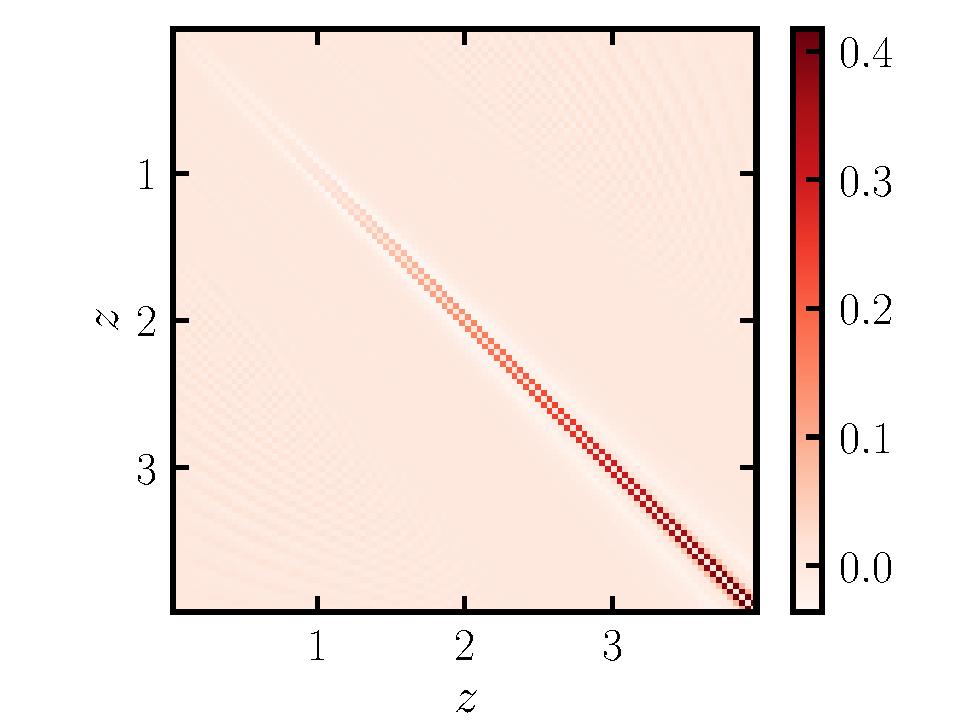
\includegraphics[width=1.\textwidth]{./corr_CV_0}
          \caption{Correlation matrix associated with the cosmic-variance contribution to the total $N(z)$ covariance for the first tomographic bin of the HSC data.}\label{fig:CV}
        \end{figure}
        The analysis presented in Section \ref{sec:hsc} will make use of a measured redshift distribution estimated from the COSMOS 30-band catalog \cite{2016ApJS..224...24L}, as was done in \cite{1912.08209}. The main sources of uncertainty for this measurement are cosmic variance in the COSMOS field, shot noise and additional uncertainty in the photometric redshifts used to assign galaxies to different bins. Here we will associate each of this sources to a separate covariance that will be added in quadrature to form the final ${\sf C}_N$. There is a fourth source of uncertainty that we do not address here: although the redshifts provided in the COSMOS 30-band catalog have a high accuracy, they are photometric and therefore subject to potential biases. This has been identified as an important source of the relative differences between ongoing cosmic shear surveys \citep{2020A&A...638L...1J}. Calibrating this bias or incorporating it into the $N(z)$ error model is an important task that requires a detailed study of the COSMOS 30-band sample, and that we leave for future work.
        
        The sample variance uncertainties are caused by the fluctuations in the matter density traced by galaxies in the particular sky patch. The corresponding covariance would ideally be estimated from simulations including both non-linear gravitational clustering and a realistic model of the galaxy-halo connection for the specific galaxy sample under study. For simplicity in this proof-of-concept analysis we instead use an analytical model for the $N(z)$ covariance. Although less precise than a simulation-based calculation, this approach was shown by \cite{2004.09542} to provide a reasonable prediction for the redsthift distribution uncertainties.

        The covariance matrix element between two tomographic bins $N^\alpha_i$ and $N^\beta_j$ is given by:
        \begin{equation}\label{eq:nz_cv}
          {\sf C}_{N,{\rm CV}}^{(i\,\alpha),(j\,\beta)}=\frac{N^\alpha_iN^\beta_j}{2\pi^2} \int_0^\infty dk_\parallel \cos(k_\parallel(\chi_\alpha-\chi_\beta))\int_0^\infty dk_\perp k_\perp W_\alpha(k_\parallel,k_\perp)W_\beta(k_\parallel,k_\perp)P_{gg}({\bf k}),
        \end{equation}
        where $\chi_\alpha$ is the radial comoving distance to redshift $z_\alpha$, and we model the galaxy power spectrum using the Kaiser formula \cite{1987MNRAS.227....1K} accounting for redshift-space distortions:
        \begin{equation}
          P_{gg}({\bf k},z)=\left(b_g(z)+f(z)\frac{k_\parallel^2}{k^2}\right)^2\,P_{mm}(k,z),
        \end{equation}
        where $f(z)$ is the logarithmic growth rate and $b_g(z)$ is the linear galaxy bias. Following the results of \cite{1912.08209}, appropriate for the magnitude-limited sample studied here, we assume a redshift dependence for $b_g$ given by $b_g(z) = 0.95/D(z)$, with $D(z)$ the linear growth factor. $P_{mm}(k)$ is the real-space non-linear matter power spectrum, which we model via the HALOFIT parametrization \cite{2003MNRAS.341.1311S,2012ApJ...761..152T}.

        The overlapping deep HSC patch covering the COSMOS 30-band footprint used to measure the redshift distribution in this work covers a total area of $A_{\rm sky} = 1.7 \ {\rm deg}^2$. Modelling this patch as a disc of radius $\theta_{\rm sky}=0.73^\circ$, the corresponding window function in Eq. \ref{eq:nz_cv} is given by
        \begin{equation}
          W_\alpha(k_\parallel,k_\perp)=j_0(k_\parallel\Delta\chi_\alpha/2)\,\frac{2 J_1(k_\perp \chi_\alpha\theta_{\rm sky})}{k_\perp \chi_\alpha\theta_{\rm sky}},
        \end{equation}
        where $\Delta\chi_\alpha$ is the comoving width of the $\alpha$-th histogram bin, $j_0$ is the zero-th order spherical Bessel function and $J_1$ is the order-1 cylindrical Bessel function.

        We assume that the cosmic covariance between the tomographic bins is negligible, so we estimate the cosmic variance covariance matrix by treating each bin independently. Figure \ref{fig:CV} shows the correlation matrix associated with this cosmic variance contribution in the COSMOS 30-band sample for the first tomographic bin used in Section \ref{ssec:hsc.data}.
        
        The final contribution, from shot noise, is caused by the discrete nature of galaxies as a tracer of the matter fluctuations, and is simply given by
        \begin{equation}\label{eq:cov_nz_shot}
          {\sf C}^{(i\,\alpha),(j\,\beta)}_{N,{\rm SN}}=\delta_{\alpha\beta}\delta_{ij}N^\alpha_i.
        \end{equation}
        We find this contribution to be subdominant in all cases in comparison with sample variance.


        Finally we estimate the systematic error associated with the choice of photo-$z$ code as follows. Following \cite{1912.08209}, we consider  {\tt DEmP}, {\tt Ephor}, {\tt Ephor\_AB} and {\tt FRANKEN-Z} as some of the best-performing algorithms presented in \cite{2018PASJ...70S...9T}, and constitute a fair representation of the underlying photo-$z$ uncertainties. Note however that all of these codes rely on COSMOS-30 for calibration. We calculate the variance between $N(z)$s estimated from each code by stacking the redshift probability density functions (pdfs) of each source in the HSC data.  We multiply this variance by a factor $A_{\rm noise}$ and smooth it by convolving it with a Gaussian kernel with standard deviation $\sigma_z=0.1$. The resulting variance vector is added to the diagonal of the pure sample variance covariance matrix. We discuss sensitivity to some of these partially subjective choices in Section \ref{ssec:hcs.mcmc}.

    \subsubsection{External priors and smoothness}\label{sssec:theory.prior.smooth}
      In addition to information from direct measurement of the $N(z)$, it is reasonable to impose certain properties on the underlying true reshift distributions based on physical considerations. For instance, there is no reason to expect that the physics of galaxy formation should generate sharp features in the redshift evolution of the abundance of galaxies. The transition of features in the spectra of different galaxy types between photometric bands at different redshifts could induce smaller-scale fluctuations in the $N(z)$. However, for a sufficiently diverse galaxy sample, one would not expect such fluctuations on scales $\delta z\lesssim0.04$ (corresponding to $\sim100\,{\rm Mpc}$ or $\sim0.2\,{\rm Gyr}$ at $z\sim1$). It is therefore a reasonable proposition to impose a certain degree of smoothness on the redshift distributions, which can be achieved through a purposely defined Gaussian prior. Applying these types of priors is admittedly a subjective choice to some extent, and we will study its impact on our results in Section \ref{ssec:hcs.mcmc}.
      
      One common way to impose smoothness on a function $f(x)$ is to penalize large values of its first derivative via a Gaussian prior of the form $p(f)\propto\sum_x\exp\left[-(f'(x))^2/(2\sigma_1^2)\right]$. In the discrete formalism used here, using first-order finite differences, this is equivalent to imposing a Gaussian prior on $\vN$ with zero mean ($\vN_P=0$) and an inverse covariance given by:
      \begin{equation}\label{eq:prior_1st}
        {\sf C}^{-1}_P=\frac{1}{\sigma_1^2}\sum_\alpha {\bf v}^{1T}_\alpha{\bf v}^1_\alpha,
      \end{equation}
      where
      \begin{equation}
        ({\bf v}^1_\alpha)_\beta=\left\{
        \begin{array}{ll}
          1  & {\rm if}\,\,\, \alpha=\beta+1\\
          -1  &  {\rm if}\,\,\, \alpha=\beta\\
          0 & {\rm otherwise}
        \end{array}\right.
      \end{equation}
      To understand this, note that, using finite differences, the derivative of $\vN$ is approximately $\vN'\propto {\bf v}^{1T}\vN$.

      The prior in Eq. \ref{eq:prior_1st} effectively penalizes large deviations between adjacent elements of $\vN$. This can be generalized to include all possible pairs of elements as
      \begin{equation}\label{eq:smooth1}
        {\sf C}^{-1}_P=\sum_{n=1}\sum_{\alpha}p_n\,{\bf v}^{n\,T}_\alpha{\bf v}^n_\alpha,
      \end{equation}
      where
      \begin{equation}
        ({\bf v}^n_\alpha)_\beta=\left\{
        \begin{array}{ll}
          1  & {\rm if}\,\,\, \alpha=\beta+n\\
          -1  &  {\rm if}\,\,\, \alpha=\beta\\
          0 & {\rm otherwise}
        \end{array} \right..
      \end{equation}
      The prefactor $p_n$ penalizes differences between neighbors of order $n$, and should therefore be a monotonically decreasing function of $n$ (since there should be no correlation between widely separated histogram bins). We therefore choose a functional form
      \begin{equation}
        p_n=A_{\rm smooth}\,{\rm exp}\left[-\frac{1}{2}\left(n\frac{\Delta z}{\Delta z_{\rm thr}}\right)^2\right],
      \end{equation}
      where $\Delta z$ is the redshift separation between neighbouring histogram bins, and $\Delta z_{\rm thr}$ marks the redshift separation beyond which different elements of the $N(z)$ are expected to be uncorrelated. Our fiducial analysis uses $A_{\rm smooth}=1$ and $\Delta z_{\rm thr}=0.06$. These values were empirically chosen to cause a mild smoothing of the redshift distribution directly measured from the COSMOS catalog. As we discuss in Section \ref{ssec:hcs.mcmc}, this choice has no practical impact on the final results.
    
    \subsubsection{Up-sampling}\label{sssec:theory.prior.ups}
      Depending on the size of the spectroscopic sample used to estimate the initial redshift distribution, the measured $\hat{\vN}$ may be provided with a relatively coarse redshift spacing to reduce the jaggedness in the fiducial $N(z)$. However, it may often be desirable to explore the impact of variations in the $N(z)$ on scales smaller than that, which implies artificially increasing the size of $\vN$ by up-sampling the original distributions into a finer grid of $z$.
      
      This up-sampling can be done in different ways, but in general can be expressed as a linear operation of the form
      \begin{equation}
        \vN_{\rm fine}={\sf O}\,\vN_{\rm coarse}.
      \end{equation}
      The prior covariance of $\vN_{\rm fine}$ is then related to that of $\vN_{\rm coarse}$ via the bilinear operation
      \begin{equation}
        {\sf P}_{\rm fine}={\sf O}\,{\sf P}_{\rm coarse}\,{\sf O}^T.
      \end{equation}
      
      For nearest-neigh interpolation, the linear kernel $O_{\mu\alpha}$ is simply $O_{\mu\alpha}=\delta_{\alpha\alpha_\mu}$, where $\alpha_\mu$ is the index of the coarse redshift distribution element that lies closest to the finer grid element with index $\mu$. Higher-order interpolation methods can be described in terms of different kernels. In practice, the easiest procedure is to simply apply the same interpolating function used to up-sample $\vN$ to all the rows and then all the columns of ${\sf P}_{\rm coarse}$.
      
      The original $N(z)$s obtained from the COSMOS catalog were measured in bins of $\Delta z=0.04$ in the range $z\in(0,4)$. We up-sampled them using linear interpolation by a factor $N_{\rm up}=3$ to a resolution $\Delta z=0.0133$. For the total 4 bins used in this analysis, the final up-sampled $\vN$ has 1200 elements.

  \section{Appplication to galaxy clustering in HSC}\label{sec:hsc}
    \an{Some citations are currently missing but I will put them in later.} \da{I added a few, have a look.}
    We apply the method outlined in the previous section to the data presented in Ref.~\cite{1912.08209}. This work measured the angular galaxy clustering power spectrum from the first data release (PDR1) of the Hyper Suprime-Cam survey, described in detail in \cite{2018PASJ...70S...8A,2018PASJ...70S..25M,2018PASJ...70S...5B}. In the following, we give a very brief summary of the methodology employed in Ref.~\cite{1912.08209} and refer the reader to the original paper for further details.
    
    \subsection{Background theory}\label{ssec:hsc.theory}
      The angular clustering power spectrum for galaxies in redshift bins $i$, $j$ with can be modeled using the Limber approximation as \cite{1953ApJ...117..134L, 1992ApJ...388..272K, Kaiser:1998}
      \begin{equation}\label{eq:cell_gg_limber}
        C^{ij}_\ell = \int \mathrm{d}z\,\frac{H(z)}{\chi^2(z)} p^i(z)p^j(z)\,P_{gg}\left(z,k=\frac{\ell+1/2}{\chi(z)}\right),
      \end{equation}
      where $P_{gg}(z,k)$ denotes the underlying 3D galaxy power spectrum, $\chi(z)$ is the comoving distance and $H(z)$ denotes the Hubble parameter at redshift $z$. $p^i(z)$ is the redshift probability distribution of bin $i$ normalized to unit area, and is therefore related to the unnormalized distribution via
      \begin{equation}
        p^i(z)=\frac{N_i(z)}{\int dz' N_i(z')}=\frac{\sum_\alpha N^\alpha_i\phi_\alpha(z')}{\sum_\alpha N^\alpha_i\int dz\phi_\alpha(z')}.
      \end{equation}
      The simplicity with which the redshift distribution amplitudes $N_i^\alpha$ enter the prediction for the angular power spectrum in Eq.~\ref{eq:cell_gg_limber}, facilitates the computation of the ${\sf T}$ matrix defined in Eq. \ref{eq:Tmat}. 

      Following Ref.~\cite{1912.08209} we estimate the theoretical prediction for the galaxy power spectrum $P_{gg}(z,k)$ within the halo model combined with halo occupation distribution (HOD) modeling \cite{2000MNRAS.318.1144P,2002PhR...372....1C,2002ApJ...575..587B,2005ApJ...633..791Z,2013MNRAS.430..725V}. Details about HOD parametrizations can be found in these references, and we only provide a succinct description relevant to the present analysis here

      The galaxy power spectrum receives contributions from the so-called 1-halo and 2-halo terms:
      \begin{equation}
        P_{gg}(z,k) = P_{gg,{\rm 1h}}(z,k) + P_{gg,{\rm 2h}}(z,k),
      \end{equation}
      where
      \begin{align}
        & P_{gg,{\rm 1h}}(k)=\frac{1}{\bar{n}_g^2} \int \mathrm{d}M\,\frac{\mathrm{d}n}{\mathrm{d}M} \bar{N}_c\,\left[\bar{N}_s^2u_s^2(k)+2\bar{N}_su_s(k)\right],\\
        & P_{gg,{\rm 2h}}(k)=\left(\frac{1}{\bar{n}_g} \int \mathrm{d}M\,\frac{\mathrm{d}n}{\mathrm{d}M}\,b_h(M)\,\bar{N}_c\,\left[1+\bar{N}_su_s(k)\right]\right)^2\,P_{\rm lin}(k).
      \end{align}
    
      Here, $\mathrm{d}n/\mathrm{d}M$ is the halo mass function for halo mass $M$, $b_h(M)$ is the linear halo bias, $\bar{N}_c(M)$ and $\bar{N}_s(M)$ are the mean number of central and satellite galaxies in halos of mass $M$, $u_s(k)$ is the Fourier transform of the satellite density profile, and $P_{\rm lin}(k)$ is the linear matter power spectrum. The number density of galaxies is calculated as 
      \begin{equation}
        \bar{n}_g=\int \mathrm{d}M\,\frac{\mathrm{d}n}{\mathrm{d}M}\bar{N}_c(M)\left[1+\bar{N}_s(M)\right].
        \label{eq:ng_hod}
      \end{equation}    
    
      As in \cite{1912.08209}, we parametrize the number of centrals and satellites as a function of mass as:
      \begin{align}
        &\bar{N}_c(M)=\frac{1}{2}\left[1+{\rm erf}\left(\frac{\log_{10}(M/M_{\rm min})}{\sigma_{\log M}}\right)\right],\\
        &\bar{N}_s(M)=\Theta(M-M_0)\left(\frac{M-M_0}{M_1'}\right)^\alpha,
      \end{align}
      where $\Theta(x)$ is the Heavyside step function, and we model the distribution of satellites to follow that of the dark matter, given by a truncated Navarro-Frenk-White profile \cite{Navarro:1996}. The choices of mass function parametrization, halo bias and concentration-mass relation used here follow the same models used in \cite{1912.08209}, namely the mass function and halo bias of \cite{Tinker:2010}, and the concentration-mass relation of \cite{Duffy:2008} for a spherical overdensity halo masses with an overdensity parameter $\Delta=200$ with respect to the matter density.
 
      The HOD model is defined by three characteristic masses, $M_{\rm min}$, $M_0$ and $M_1$. We model the redshift dependence of these masses as a linear Taylor expansion in the scale factor around the mean redshift of the sample $z_p=0.65$ as
      \begin{equation}
        \log_{10}{M_x(z)} = \mu_x + \mu_{x, p} \left(\frac{1}{1+z} - \frac{1}{1+z_{p}}\right).
      \end{equation}
      where $x$ is $\mathrm{min}$, 0 or 1.
    
      Besides these HOD parameters, the analysis of \cite{1912.08209} marginalized over uncertainties in the redshift distribution using the shift-width parametrization of Eq. \ref{eq:photo-z-model}, including two additional shift and width parameters per redshift bin. For the four redshift bins described used in this example, the complete set of 14 free parameters is thus
      \begin{equation}
        \vec{\theta}=\{\mu_{\rm min},\,\mu_{{\rm min},p},\,\mu_0,\,\mu_{0,p},\,\mu_1,\,\mu_{1,p},\,\Delta z_{\{1,2,3,4\}},\,z_{w,\{1,2,3,4\}}\}.
      \end{equation}

    \subsection{The HSC dataset}\label{ssec:hsc.data}
      The Hyper-Suprime Cam survey is an on-going photometric galaxy survey survey focused mainly on weak gravitational lensing. The analysis in Ref.~\cite{1912.08209} is based on the publicly-available HSC DR1 data \cite{2018PASJ...70S...8A}, whose so-called wide fields cover approximately 108 square degrees on the sky, subdivided into seven distinct patches. Ref.~\cite{1912.08209} used these data to compute spherical harmonic galaxy clustering power spectra for four tomographic redshift bins between $z=0.15$ and $z=1.5$, taking both auto- and cross-correlations into account. These power spectra have been corrected for observational and extragalactic systematics by deprojection at the map-level \cite{2019MNRAS.484.4127A}. We also used the same scale cuts described in \cite{1912.08209}. Finally, following Ref.~\cite{2019PASJ...71...43H}, photometric redshift distributions have been estimated by cross-matching HSC galaxies to galaxies in the COSMOS 30-band photometric catalog presented in Ref.~\cite{2016ApJS..224...24L}.

    \subsection{Validating the linear expansion}\label{ssec:hsc.lin}
      \begin{figure}[ht]
        \centering
        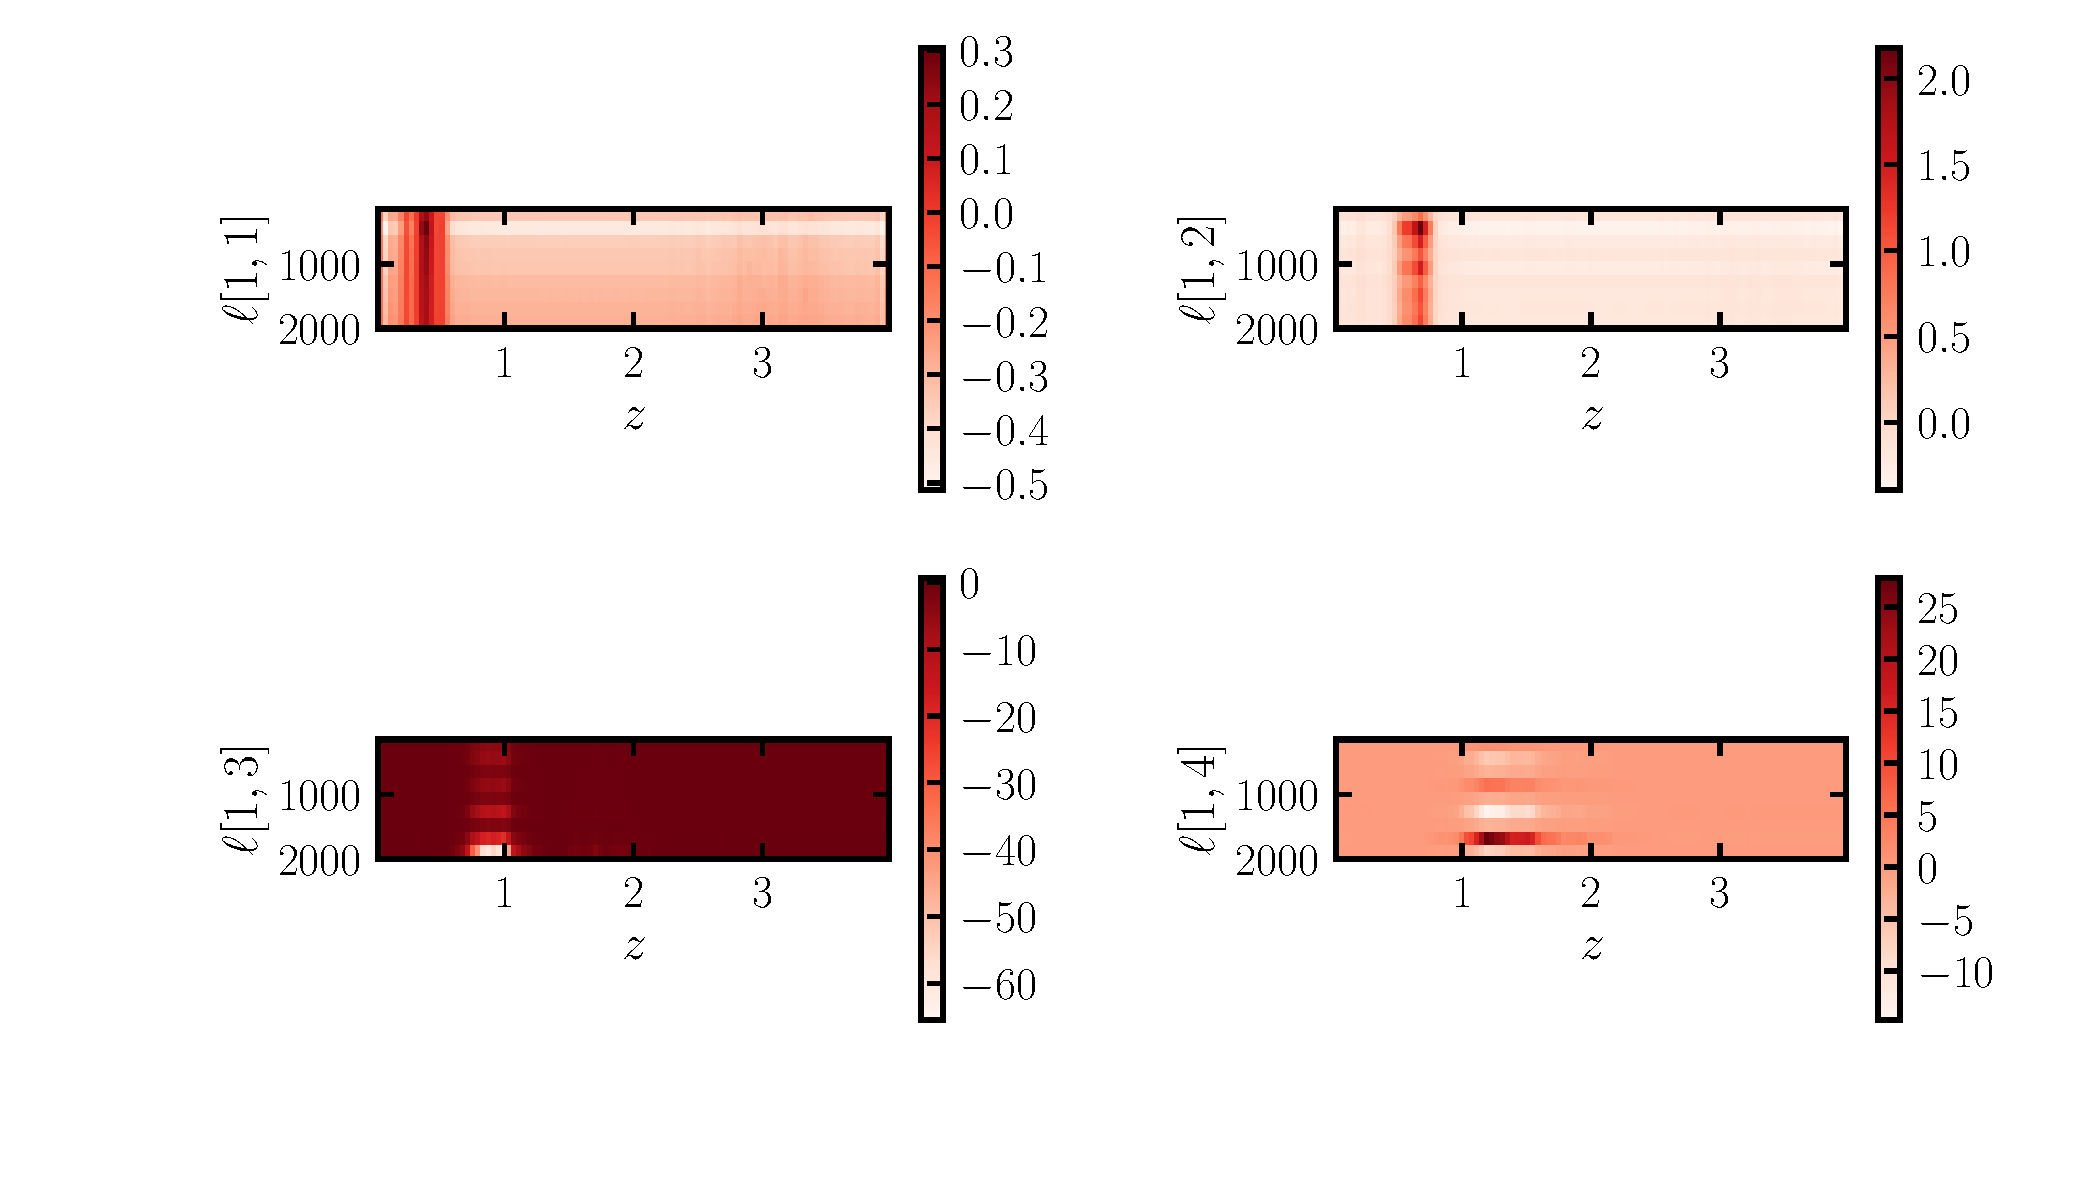
\includegraphics[width=1.\textwidth]{./Tmat}
        \caption{Visualization of the linear derivative matrix ${\sf T} = {\partial \vt}/{\partial \vN}$ divided by the angular power spectrum $C_{\ell}$ for all cross-correlation pairs between the first tomographic bin and all four others.} \label{fig:Tmat}
      \end{figure}

      \begin{figure}[ht]
        \centering
        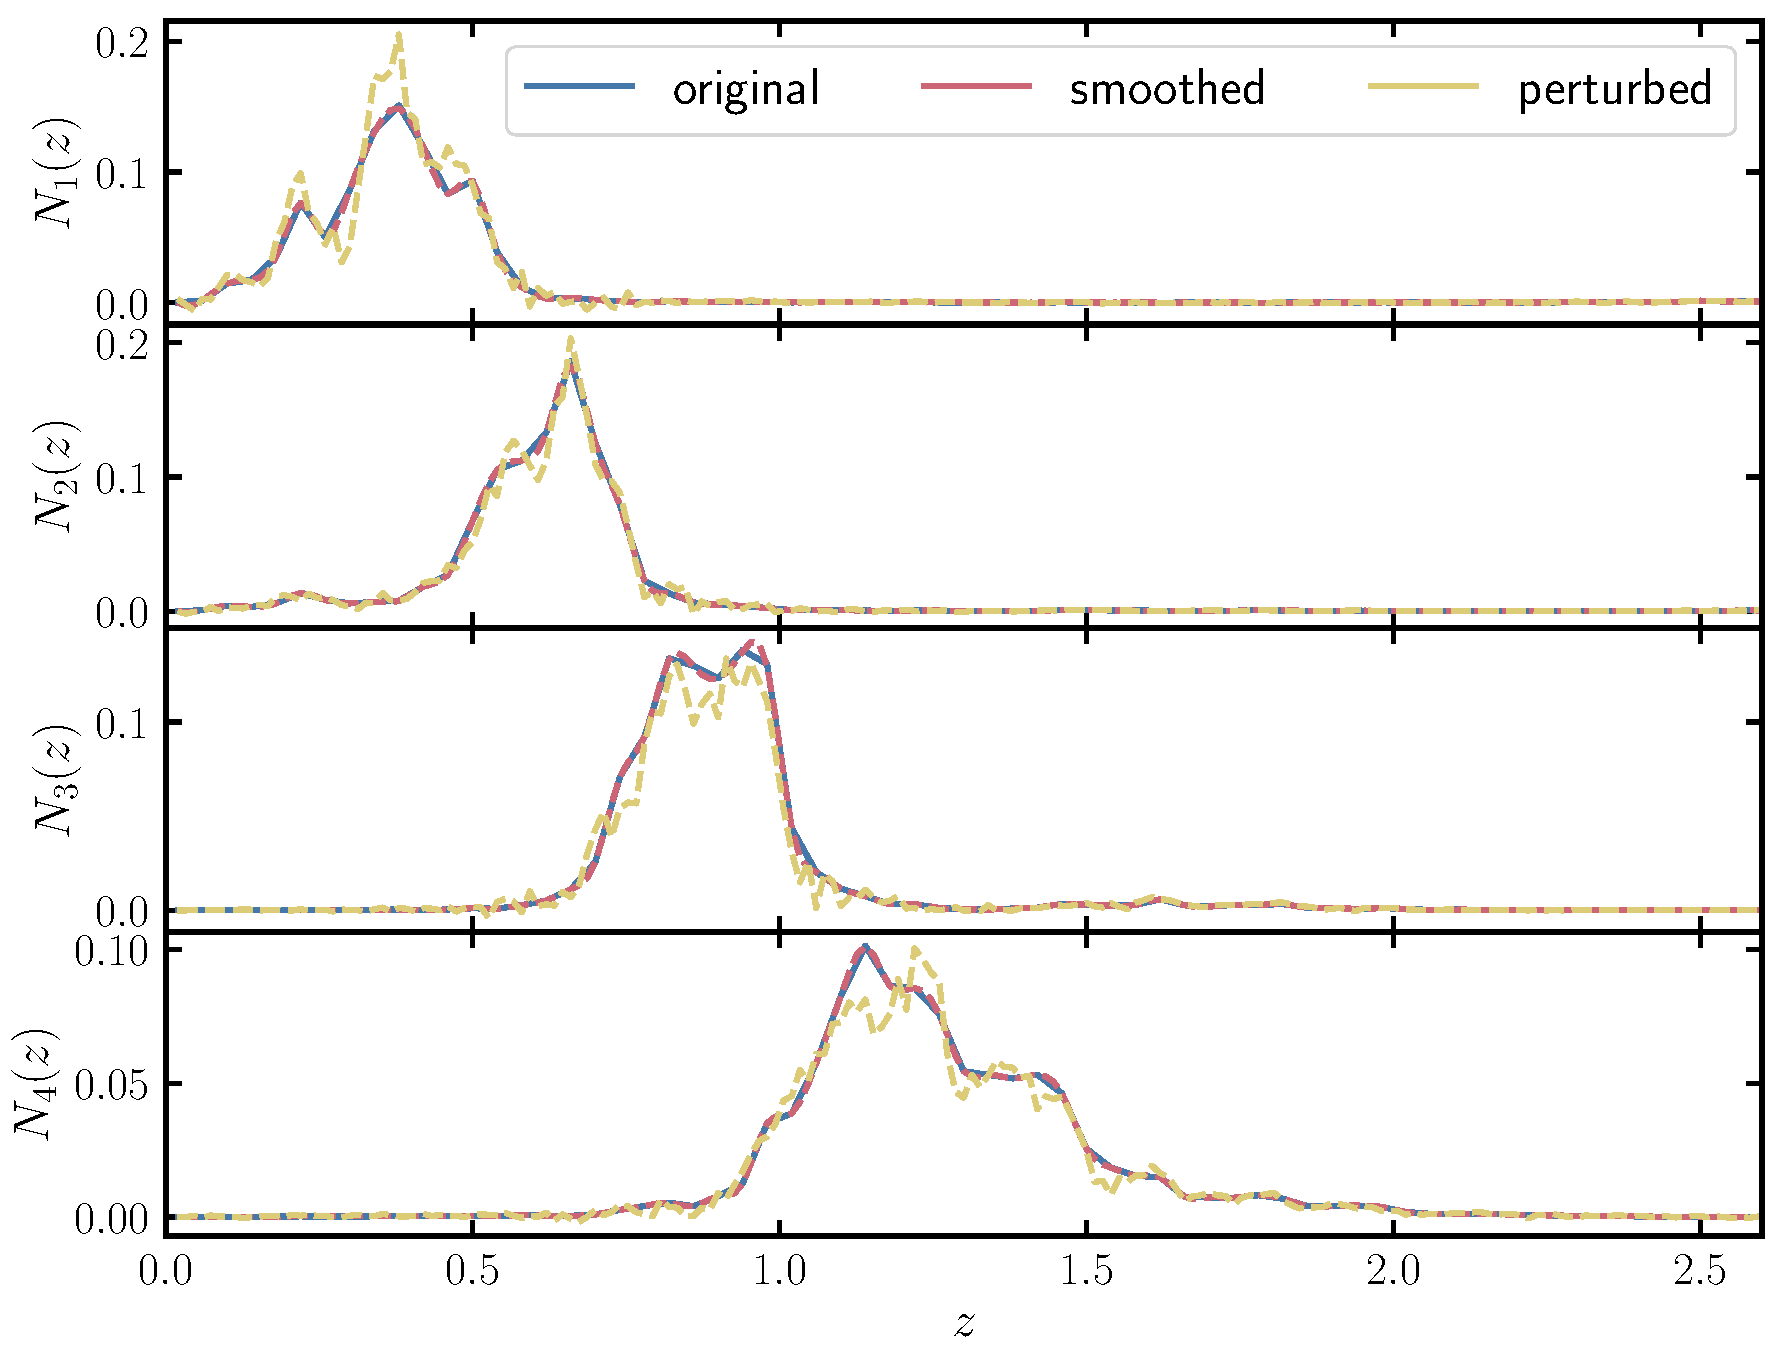
\includegraphics[width=1.\textwidth]{./Nzs}
        \caption{Photometric redshift distributions $N(z)$ of the four tomographic HSC bins. The \textit{red} curves show the default values used in the full HSC analysis \cite{1912.08209}, while the \textit{blue} curves show their smoothed and up-sampled version used in this work. The \textit{green} show a random Gaussian draw from the smoothing prior described in Section~\ref{sssec:theory.prior.smooth}.}\label{fig:Nzs}
      \end{figure}

      \begin{figure}[ht]
        \centering
        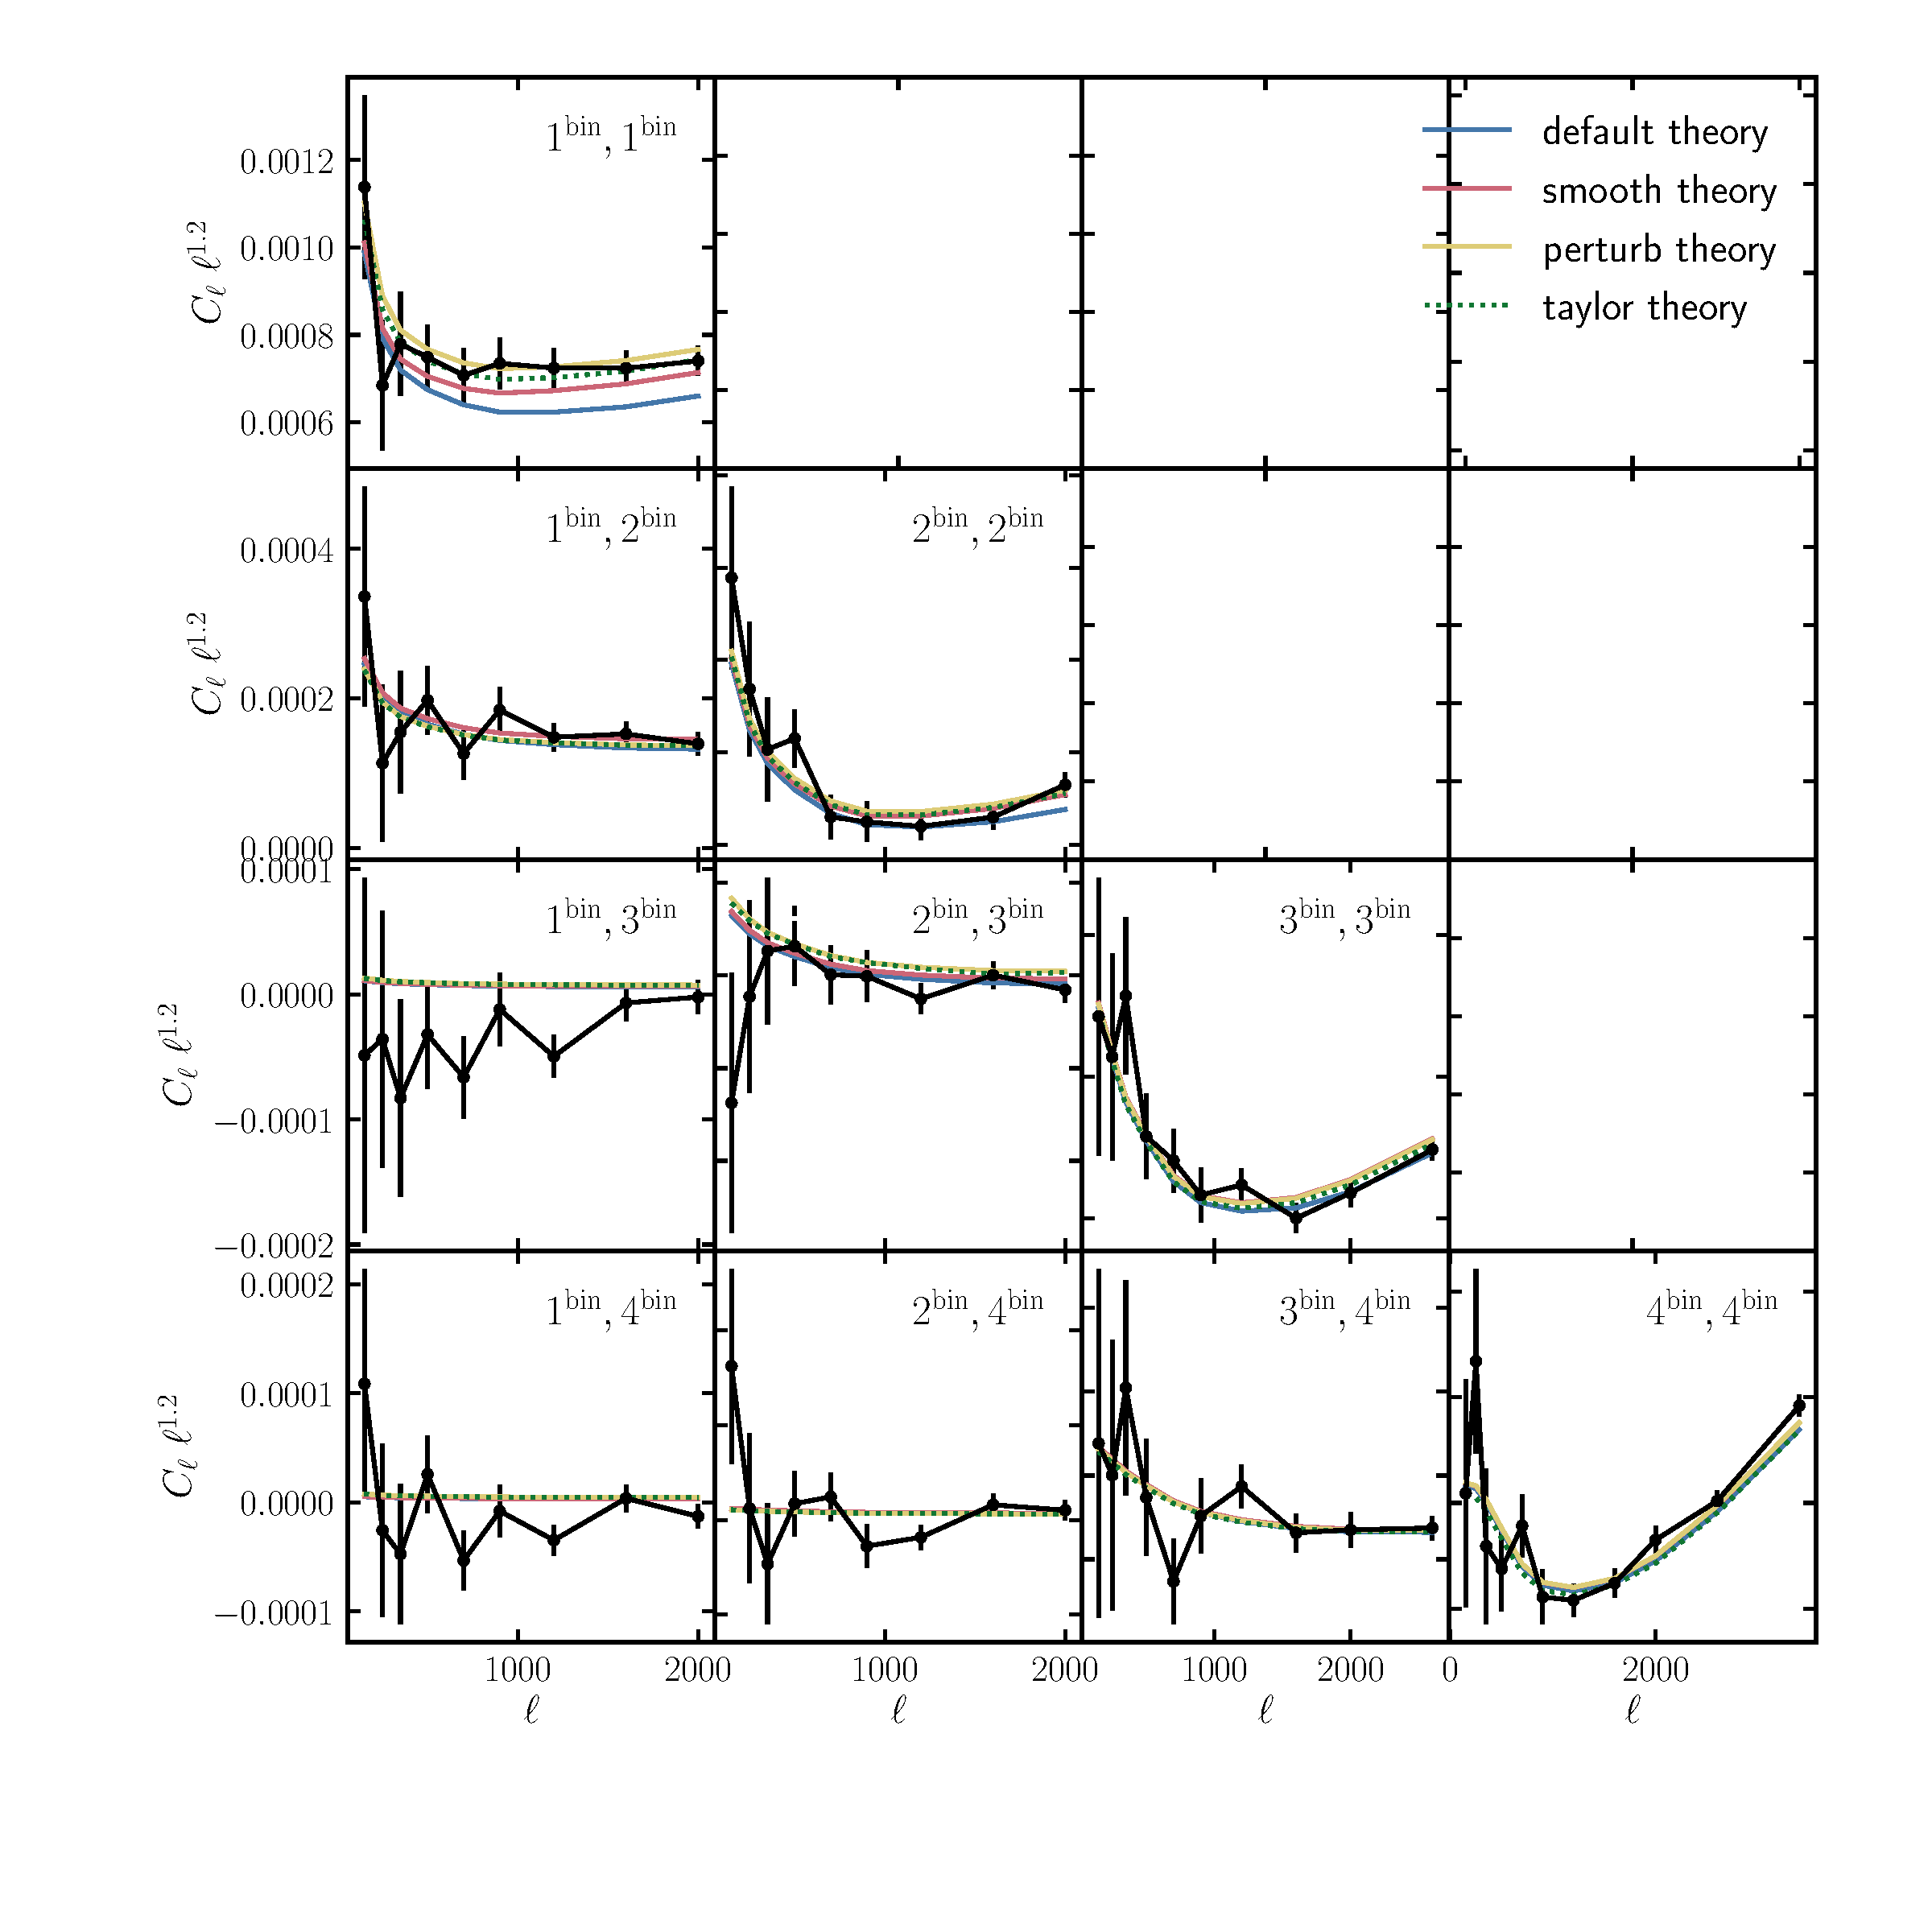
\includegraphics[width=1.\textwidth]{./Cls}
        \caption{Galaxy power spectrum with subtracted shot noise, $C_\ell^{gg}$, between the four tomographic bins. The \textit{black} curves illustrate the HSC-measured power spectrum and error bars, while the \textit{red} curves show the $C_\ell$s computed using the posterior mean values of the 6 HOD parameters from the full HSC analysis \cite{1912.08209}. In \textit{green}, we show the angular power spectrum obtained by using the smoothed $N(z)$ distributions (see Fig.~\ref{fig:Nzs}). The \textit{blue} curves correspond to the exact calculation of the $C_\ell$s using the perturbed $N(z)$ values in Fig.~\ref{fig:Nzs}, and the \textit{lightblue} dotted lines show the power spectra derived via Taylor expansion: $C_\ell' = C_\ell + {\sf T} \left(\vN' - {\vN} \right)$. \da{Isn't the fit of the blue line to the data super horrible in the first bin? Maybe the NG covariance actually allows this...}}\label{fig:Cls}
      \end{figure}

      In this section, we study how the linear approximation performed via the derivative matrix ${\sf T}$ (defined in Eq. \ref{eq:Tmat}) compares with the exact $C_\ell$ calculation.
      
      The derivative matrix can be seen in Fig.~\ref{fig:Tmat} for the first tomographic bin and its cross-correlations with all four bins in the HSC data, i.e. the tomographic pairs [1,1], [1,2], [1,3], and [1,4]. The rows of the matrix correspond to the $\ell$ multipole bandpowers available for each pair, and the columns to the 300 equally-spaced redshift samples of $N(z)$ between $z = 0$ and $z = 4$. We can notice that as we move to pairs with bins at higher redshifts, the corresponding block of ${\sf T}$ peaks at a redshift column roughly corresponding to the maximum of the deepest distribution of the pair.
      
      These $N(z)$s are shown in Fig.~\ref{fig:Nzs}. We obtain the fiducial ``measured'' distributions $\hat{\vN}$, shown in solid blue in the Figure, using the COSMOS 30-band catalog re-weighted to account for the different colour space distribution of that sample using a nearest-neighbours approach as described in \da{cite}. The figure also shows the {\sl smoothed} distribution $\bar{N}$ in dashed red, defined in Eq. \ref{eq:priorcov}. Our choice of smoothing prior has only a mild effect on the original redshift distribution, mostly removing sharp features at the edges of adjacent $N(z)$ measurements. Also shown in solid yellow is a realization of $\vN$ drawn from a multivariate Gaussian distribution with a mean given by the red line and a covariance given by ${\sl P}$ in Eq. \ref{eq:priorcov} \da{Is this true? If the smoothing prior has any relevance, then it should only allow "smooth" fluctuations. Also, the third bin is kind of suspicious in that all the fluctuations seem to be low.}

%      \bh{It is a Gaussian draw from the inverted smoothing prior multiplied by 0.6, see this code %line\url{https://github.com/damonge/WeePeeZee/blob/ce50049c6be90ca40b3a903ba782d8bff4b46c78/create_sac%c.py##L246}}
%      % , and \\ \texttt{calculate\_smooth\_s\_and\_prior.py} for details on the smoothing prior but %it should be same as the equation being referenced}.
      
      The angular power spectra, $C_\ell$, estimated for the same three sets of $N(z)$s are shown in Fig.~\ref{fig:Cls} using the same color scheme. The figure also shows the comparison between the exact prediction for the $N(z)$s (yellow line) and the linear prediction around the smoothed distribution using the derivative matrix, ${\sf T}$, (\textit{dotted light-blue line}). We find that the two are in reasonably good agreement given the statistical uncertainties in the data. This may not be the case for future datasets with higher statistical power, although the expectation is that those data will be accompanied by larger spectroscopic samples \da{cite some of the Euclid efforts?} needed to reduce systematic photo-$z$ uncertainties. It is worth noting that the agreement between exact prediction and linear model is noticeably worse for auto-correlations. As described in Appendix \ref{app:autos}, this is due to the fact that a single $N(z)$ enters the corresponding auto-correlation quadratically, making higher-order terms in Taylor expansion more relevant than in the case of cross-correlations.


      The $\chi^2$ values for all four curves with respect to the HSC data are shown in Table~\ref{tab:lin}. Comparing the $\chi^2$ values for the original and smoothed $N(z)$ distributions, we notice that they decrease for both the HSC covariance matrix and also for the marginalized one. As expected, perturbing the photometric distributions gets penalized, but the change in the $\chi^2$ value is much larger for the original HSC covariance, which indicates that the marginalized covariance is more lenient in allowing small (and expected) $N(z)$ fluctuations. The difference between the last two lines suggests that the Taylor expansion works sufficiently well, as the difference in $\chi^2$ is negligible. Finally, comparing the $\chi^2$ for the new and old covariances, we are led to conclude that the new covariance provides a better fit to the data. We note that we have fixed the values of all the shift and width parameter to be zero and set the 6 HOD parameters to their fiducial values of
      \begin{equation}\label{eq:par_fid}
        (\mu_{\rm min},\mu_{{\rm min},p},\mu_0,\mu_{0,p},\mu_1,\mu_{1,p})=(11.88,-0.5,5.7,2.5,13.08,0.9).
      \end{equation}
      
      These HOD values correspond to the posterior means reported in Ref. \cite{1912.08209}. For the smoothed and perturbed $N(z)$ values only, we minimize the likelihood to find the best fit values for the 2 HOD parameters $\mu_1$ and $\mu_{1,p}$, obtaining 13.05 and 0.79, respectively \da{It's not clear if you get the same values for both the smoothed and perturbed $N(z)$s (which would be weird) or just for one of them. It's also not clear if you're saying that you did this for the results in Table \ref{tab:lin} or just now.}. The ratio of  the original HSC precision matrix to the marginalized $N(z)$ one \da{Not clear at all how you calculate this number or why it's relevant} is  $1.15^{\nu_{\rm tot}}$, where $\nu_{\rm tot} = 94$ is the number of total degrees of freedom of the system (i.e. size of the $C_\ell$ vector for all cross correlations between the tomographic bins).

      \begin{table}
        \begin{center}
          \begin{tabular}{l| c c }
            \hline\hline
            Model & HSC cov. & Marginalized $N(z)$ cov. \\ [0.5ex]
            \hline
            $\chi^2$, original $N(z)$, exact $C_\ell$ & 98.97 & 88.97 \\ 
            $\chi^2$, smoothed $N(z)$, exact $C_\ell$ & 91.33 & 86.44 \\
            $\chi^2$, perturbed $N(z)$, exact $C_\ell$ & 99.78 & 89.57 \\
            $\chi^2$, perturbed $N(z)$, $C_\ell(\bar{\vN}) + {\sf T} \Delta \vN$ & 100.62 & 89.64 \\
            \hline
            \hline
          \end{tabular}
        \end{center}
        \caption{$\chi^2$ values with respect to the HSC data of the four curves shown in Fig.~\ref{fig:Cls} using the original covariance used in the HSC analysis and the marginalized $N(z)$ covariance developed in this work.}\label{tab:lin}
      \end{table}

    \subsection{Impact of N(z) uncertainties on final parameters}\label{ssec:hcs.mcmc}
      \begin{figure}
        \centering
        \begin{subfigure}{.5\textwidth}
          \centering
          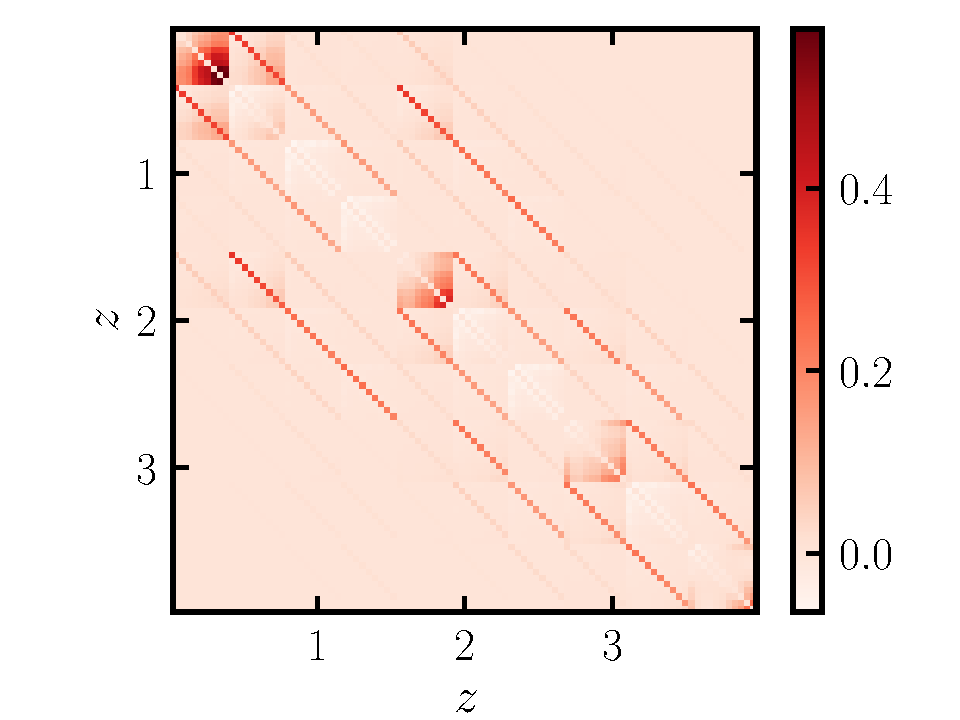
\includegraphics[width=1.\linewidth]{./corr_data}
        \end{subfigure}%
        \begin{subfigure}{.5\textwidth}
          \centering
          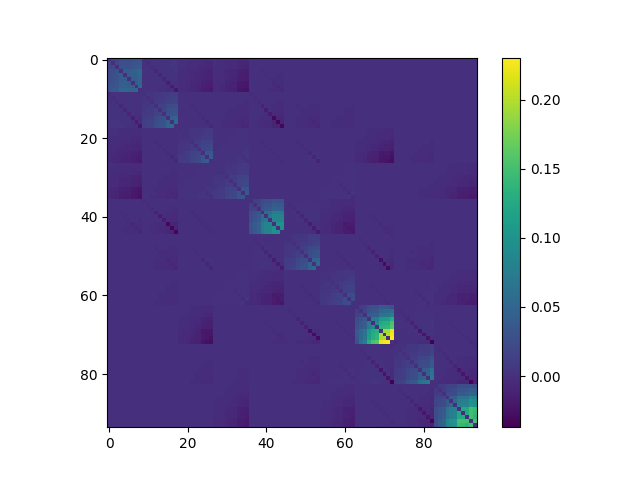
\includegraphics[width=1.\linewidth]{./corr_diff}
        \end{subfigure}
        \caption{Correlation matrix of the original HSC dataset (\textit{left} panel) and difference between the original and the marginalized (this work) correlation matrices (\textit{right} panel). Most of the effect of marginalizing for the shift and width parameters is manifested as a positive contribution to the original matrix near the diagonal (i.e. there is an increase in correlation for close redshift values). Note that we have subtracted the diagonal off the two matrices.}\label{fig:fid_marg_cov}
      \end{figure}
      \begin{figure}
        \centering  
        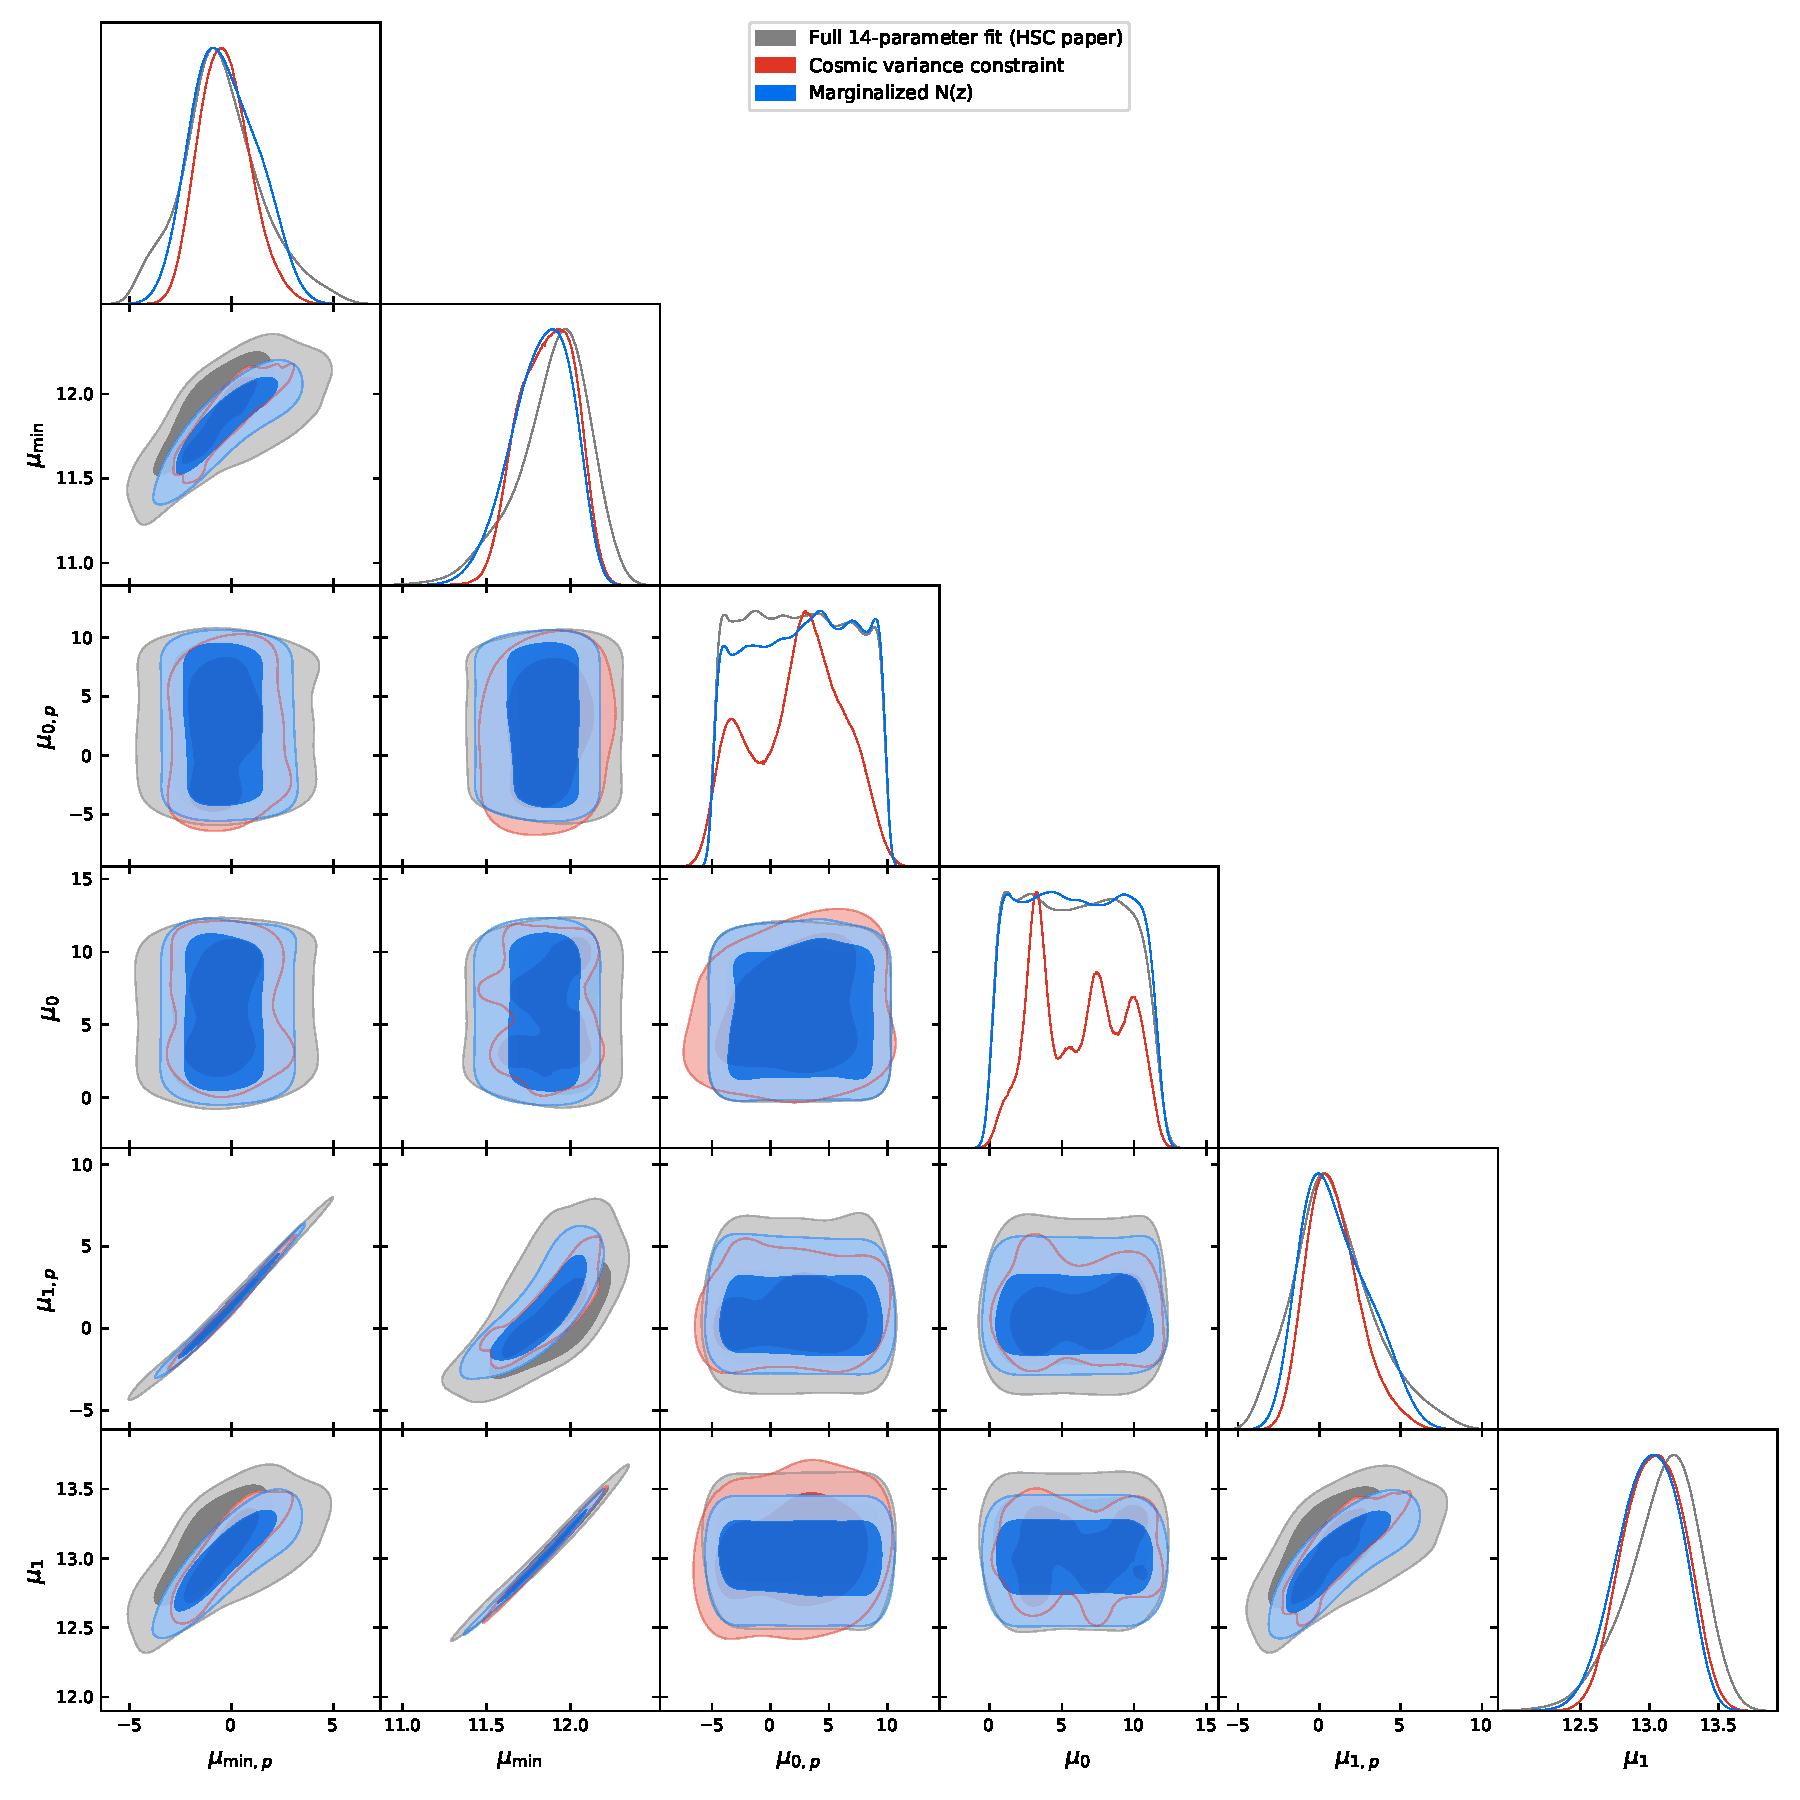
\includegraphics[width=1.\textwidth]{./triangle_fid_marg}
        \caption{Triangle plot with constraints of the 6 HOD parameters obtained using the  covariance matrix from the full 14-parameter original HSC analysis (\textit{gray contours}). The \textit{red contours} are obtained by running an MCMC chain with the original HSC covariance and a Gaussian prior on the 4 shift and 4 width parameters with a zero mean and an RMS width for each parameter determined by its statistical distribution over a number different realizations of the cosmic variance. In \textit{blue}, we show the constraints on the 6 HOD parameters obtained using the covariance matrix marginalized to account for the $N(z)$ uncertainty (i.e. without the 8 shift and width parameters). We can see that the full analysis leads to worse constraints on the parameters when compared with the marginalized covariance.} \label{fig:triangle_fid_marg}
      \end{figure}
      In this section, we summarize the main results of this paper, showing in particular the effect of marginalization of the photometric uncertainties on the final parameter constraints. In our particular case, these are the 6 HOD parameters described in Section~\ref{ssec:hsc.theory}. The ${\sf T}$ matrix used to calculate the marginalized $N(z)$ covariance was computed assuming the fiducial HOD parameters listed in Eq. \ref{eq:par_fid}.

      To study the effect on the covariance matrix of the marginalization procedure described in detail in Section~\ref{ssec:theory.nz_new}, we visualize the original correlation matrix and its difference with the marginalized matrix in Fig.~\ref{fig:fid_marg_cov}. The main difference with the original matrix is a positive contribution to the off-diagonal entries for redshift samples in close proximity.
      
      We set the free parameters of our model to the following values \da{these parameters are not defined anywhere. I think I know what they are, so I'll try to add it to section 2.}: $(A_{\rm smooth},\,A_{\rm noise},\,N_{\rm up},\,\Delta z_{\rm thr})=(1,\,4,\,3,\,0.06)$. These values were chosen so as to reduce the $\chi^2$ of the perturbed model using the marginalized covariance matrix when compared with the original covariance matrix \da{This sentence is imprecise. Presumably there's many parameter combinations that would achieve some level of reduction. As it is, the sentence reads as if you tweaked the parameters to get the result you want. I think I would remove the sentence}. The modest value of the smoothing parameter, $A_{\rm smooth}$ \da{So this is still something that confuses me: why can we say that $A_{\rm smooth}=1$ is ``small''? not sure what to compare it with, and in any case this value would depend on how the $N(z)$ is normalized. Should we say that the value was chosen to visually achieve some level of smoothing without massively changing the original $N(z)$?}, ensures that we are not oversmoothing the $N(z)$ distribution, while the choice of photometric noise as four times larger than the variance in the different photometric redshift codes provides a conservative estimate of the expected variation in $N(z)$ given the uncertainty \da{I feel like this discussion should have happened in Section 2, so I'll move it there.}.
      \begin{table}
        \begin{center}
          \begin{tabular}{c | c c c c} 
            \hline\hline
            Parameter & HSC cov. [68\%, 95\%] & CV constraints [68\%, 95\%] & Marg. $N(z)$ [68\%, 95\%] \\ [0.5ex] 
            \hline
            $\chi^2/\nu$ & 87.49/80 & 88.29/80 & 88.54/88 \\ 
            $\mu_{{\rm min},p}$ & $-0.5^{+1.7}_{-2.0}$, $^{+4.0}_{-4.0}$ & $-0.44^{+0.96}_{-1.6}$, $^{+2.9}_{-2.4}$ & $-0.3^{+1.5}_{-1.8}$, $^{+3.2}_{-2.8}$ \\ [1ex]
            $\mu_{\rm min}$ & $11.90^{+0.26}_{-0.15}$, $^{+0.39}_{-0.46}$ & $11.83^{+0.19}_{-0.15}$, $^{+0.31}_{-0.31}$ & $11.83^{+0.21}_{-0.15}$, $^{+0.32}_{-0.35}$ \\ [1ex]
            $\mu_{0,p}$ & $2.4\pm 4.3$, $^{+7.2}_{-7.0}$ & $2.5\pm 4.3$, $^{+7.1}_{-7.1}$ & $2.7^{+6.7}_{-4.4}$, $^{+6.9}_{-7.1}$ \\ [1ex]
            $\mu_{0}$ & $5.7\pm 3.3$, $^{+5.5}_{-5.5}$ & $5.8\pm 3.4$, $^{+5.5}_{-5.6}$ & $5.8\pm 3.4$, $^{+5.5}_{-5.5}$ \\ [1ex]
            $\mu_{1,p}$ & $0.9^{+2.0}_{-2.8}$, $^{+5.1}_{-4.7}$ & $0.8^{+1.0}_{-2.2}$, $^{+4.0}_{-3.0}$ & $1.0^{+1.6}_{-2.6}$, $^{+4.1}_{-3.5}$ \\ [1ex]
            $\mu_{1}$ & $13.10^{+0.30}_{-0.21}$, $^{+0.48}_{-0.54}$ & $12.99\pm 0.24$, $^{+0.41}_{-0.39}$ & $13.00^{+0.25}_{-0.21}$, $^{+0.42}_{-0.44}$ \\ [1ex]
            \hline\hline
          \end{tabular}
        \end{center}
        \caption{Minimum $\chi^2$ values (divided by the degrees of freedom) reached in each of the three MCMC runs and [68\%, 95\%] constraints on the 6 HOD parameters in the following scenarios: 1) adopting the original HSC covariance matrix with 14 parameters (6 HOD + 8 $N(z)$ ones), 2) adopting the original HSC covariance matrix with Gaussian priors on the $N(z)$ parameters determined by their statistical distributions due to cosmic variance, and 3) using the marginalized $N(z)$ covariance matrix developed in this work to constrain the 6 HOD parameters.}\label{tab:chi2_fid}
      \end{table}

      To compare the results of the automatic marginalization procedure proposed in this work with those of the original shift-width parametrization in terms of the final constraints on the 6 HOD parameters, we explore the posterior distribution of these parameters in both cases using the MCMC ensemble sampler ${\tt emcee}$ \cite{2013PASP..125..306F}. To test the convergence of the parameter chains we use a simple Gelman-Rubin convergence diagnostic after analyzing the auto-correlation statistics.

      \da{I stopped here today.}
      In Fig.~\ref{fig:triangle_fid_marg} and Table~\ref{tab:chi2_fid}, we illustrate the key  comparison between the original HSC analysis, marginalising over 8 shift-width parameters, and the marginalisation scheme developed in this paper. One can notice that the full analysis (\textit{in gray}) leads to suboptimal constraints on the parameters when compared with the marginalized covariance (\textit{in blue}) in almost all cases except for those HOD parameters which are poorly constrained by the HSC dataset to begin width. Furthermore, the proximity of the \textit{blue} and \textit{red} contours \da{We haven't really explained what the red contours are. I'll rephrase} serves both as a sanity check that our method yields physical constraints of the 6 parameters (i.e. not exceeding the cosmic variance limits) while at the same time nearly optimal such (as our inferences are always limited by cosmic variance).

      To check the robustness of our result, we furthermore run the following several tests:
      \begin{itemize}
        \item[\textbf{Test 1}:] We study the effect of the smoothing prior by turning it off, $A_{\rm smooth} = 0$.
        \item[\textbf{Test 2}:] We vary the choice for the diagonal photometric noise parameter by increasing it ten-fold, $A_{\rm noise} = 42$ \da{A much better number than 40}.
        \item[\textbf{Test 3}:] We compute the ${\sf T}$ matrix using a different set of HOD parameters perturbed by $1\sigma$ relative to the fiducial ones (listed in Section \ref{ssec:hsc.lin}) \da{We should say what the new values are and we could even put a dot in the triangle plot to show how far they are from the ML}.
      \end{itemize}
      We show the comparisons between these three tests and the fiducial marginalized $N(z)$ model in Fig. \ref{fig:triangle_marg_tests} and Table~\ref{tab:chi2_tests}. One can notice that the effect of the smoothing on the constraints is negligible, while increasing the diagonal noise weakens them. Neither of these tests changes significantly the mean of the posterior distribution. On the other hand, offsetting the HOD parameters used in the ${\sf T}$ matrix computation leads to a slight shift and broadening of the contours. This is somewhat expected, since the covariance matrix in this case is far from the favoured model parameters. This slight tension results in sub-par convergence of the chains and shifted mean posteriors \da{If convergence is really an issue we should have just run them for longer. Otherwise, I'd just remove this sentence and end up by saying that the shift/puffing is small given how wrong the new parameters are.}.
      \begin{figure}[ht]
        \centering
        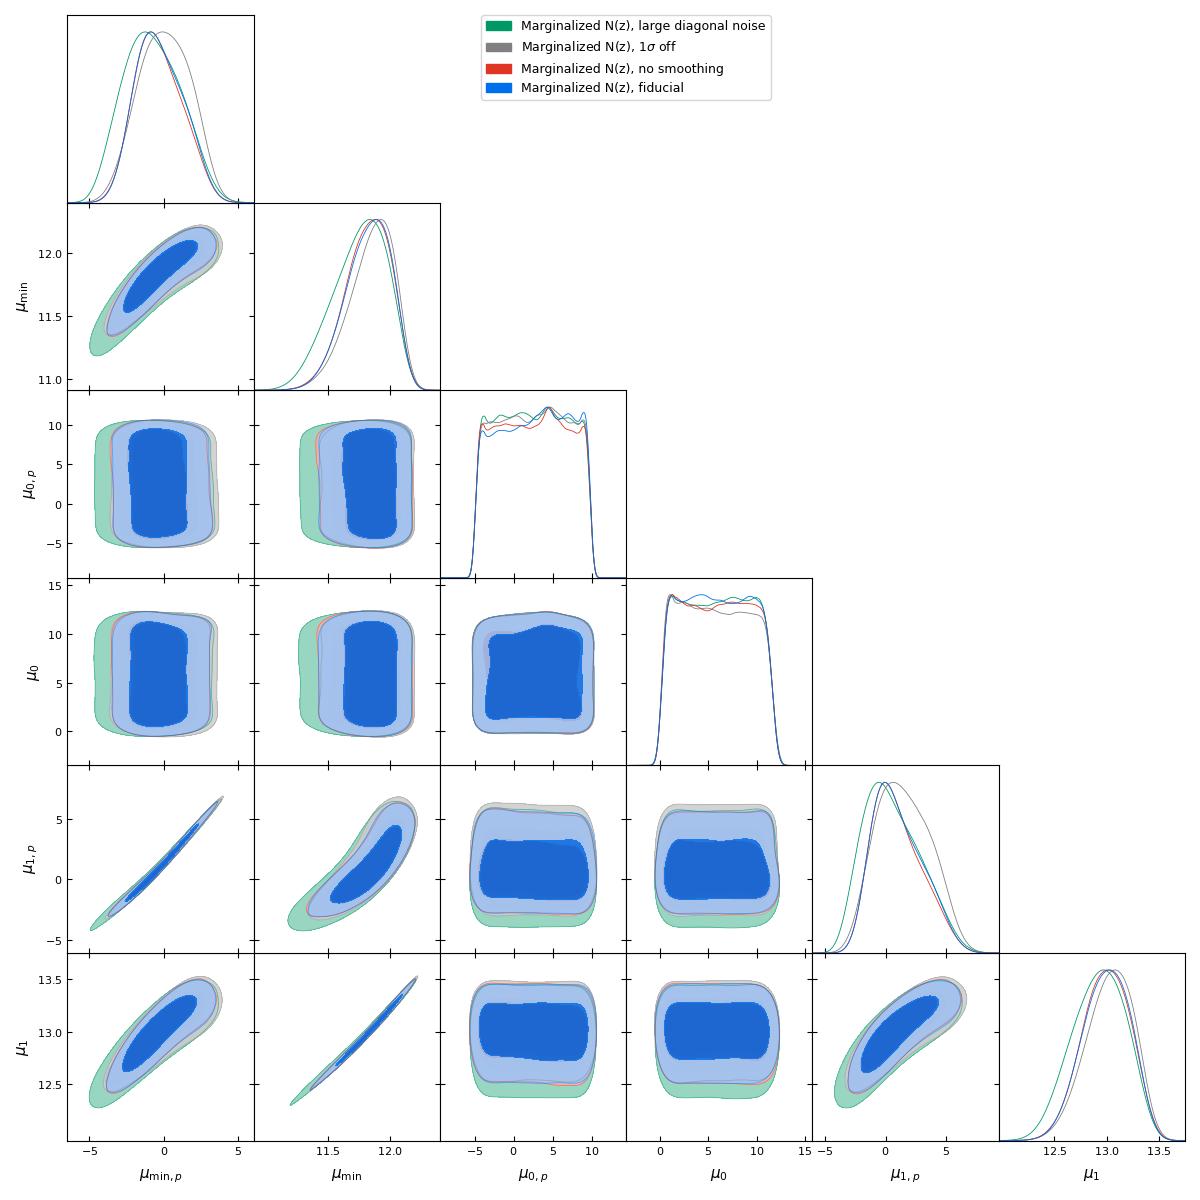
\includegraphics[width=1.\textwidth]{./triangle_marg_tests}
        \caption{Triangle plot with constraints of the 6 HOD parameters obtained using different choices for the marginalized covariance matrix: in \textit{green}, we show the result where the diagonal noise is set to a very large value ($A_{\rm noise} = 42$); in \textit{gray} is shown the case where the marginalization is performed assuming fiducial HOD-model values which are $1\sigma$ away from their posterior mean values taken from Ref.~\cite{1912.08209}; in \textit{red}, we display the case where the smoothing has been removed ($A_{\rm smooth} = 0$); and finally the \textit{blue} contours show the fiducial case with $A_{\rm noise} = 4$ and $A_{\rm smooth} = 1$.} \label{fig:triangle_marg_tests}
      \end{figure}

\iffalse
\begin{table}
\begin{center}
\begin{tabular}{c | c c c c} 
 \hline\hline
 Parameter & HSC cov. [68\%, 95\%] & CV constraints [68\%, 95\%] & Marg. $N(z)$ [68\%, 95\%] \\ [0.5ex] 
 \hline
 $\chi^2/\nu$ & 87.49/80 & --- & 88.54/88 \\ 
$\mu_{{\rm min},p}$ & $-0.5^{+1.7}_{-2.0}$, $^{+4.0}_{-4.0}$ & $-0.4^{+1.1}_{-1.4}$, $^{+2.5}_{-2.3}$ & $-0.3^{+1.5}_{-1.8}$, $^{+3.2}_{-2.8}$ \\ [1ex]
$\mu_{\rm min}$ & $11.90^{+0.26}_{-0.15}$, $^{+0.39}_{-0.46}$ & $11.86^{+0.19}_{-0.16}$, $^{+0.28}_{-0.30}$ & $11.83^{+0.21}_{-0.15}$, $^{+0.32}_{-0.36}$ \\ [1ex]
$\mu_{0,p}$ & $2.4\pm 4.3$, $^{+7.2}_{-7.0}$ & $2.1^{+4.2}_{-5.1}$, $^{+6.6}_{-7.2}$ & $2.7^{+6.7}_{-4.4}$, $^{+6.9}_{-7.1}$ \\ [1ex]
$\mu_{0}$ & $5.7\pm 3.3$, $^{+5.5}_{-5.5}$ & $6.1^{+4.6}_{-3.8}$, $^{+5.2}_{-4.8}$ & $5.8\pm 3.4$, $^{+5.5}_{-5.5}$ \\ [1ex]
$\mu_{1,p}$ & $0.9^{+2.0}_{-2.8}$, $^{+5.1}_{-4.7}$ & $0.9^{+1.3}_{-1.8}$, $^{+3.4}_{-2.9}$ & $1.0^{+1.6}_{-2.6}$, $^{+4.1}_{-3.5}$ \\ [1ex]
$\mu_{1}$ & $13.10^{+0.30}_{-0.21}$, $^{+0.48}_{-0.54}$ & $13.04\pm 0.21$, $^{+0.38}_{-0.40}$ & $13.00^{+0.25}_{-0.21}$, $^{+0.42}_{-0.44}$ \\ [1ex]
 \hline
 \hline
\end{tabular}
\end{center}
\caption{Minimum $\chi^2$ values (divided by the degrees
of freedom) reached in each of the three MCMC runs
and [68\%, 95\%] constraints on the 6 HOD parameters
in the following scenarios: 1) adopting the original
HSC covariance matrix with 14 
parameters (6 HOD + 8 $N(z)$ ones), 2)
adopting the original HSC covariance matrix 
with Gaussian priors on the $N(z)$ parameters
determined by their statistical distributions
due to cosmic variance, and 3) using the 
marginalized $N(z)$ covariance matrix developed 
in this work to constrain the 6 HOD parameters.}
\label{tab:chi2_fidd}
\end{table}
\fi

    \begin{table}
      \begin{center}
        \begin{tabular}{c | c c c c} 
          \hline\hline
          Parameter & Fiducial [68\%, 95\%] & Test 1 [68\%, 95\%] & Test 2 [68\%, 95\%] & Test 3 [68\%, 95\%] \\ [0.5ex] 
          \hline
          $\chi^2/\nu$ & 88.54/88 & 87.67/88 & 88.56/88 & 78.61/88 \\
          $\mu_{\rm min}$ & $11.83^{+0.21}_{-0.15}$, $^{+0.32}_{-0.36}$ & $11.85^{+0.22}_{-0.13}$, $^{+0.31}_{-0.37}$ & $11.83^{+0.21}_{-0.15}$, $^{+0.33}_{-0.36}$ & $11.76^{+0.26}_{-0.17}$, $^{+0.38}_{-0.43}$ \\ [1ex]
          $\mu_{0}$ & $5.8\pm 3.4$, $^{+5.5}_{-5.5}$ & $5.8^{+3.6}_{-5.2}$, $^{+5.6}_{-5.5}$ & $5.8\pm 3.4$, $^{+5.5}_{-5.5}$ & $5.9\pm 3.4$, $^{+5.5}_{-5.6}$ \\ [1ex]
          $\mu_{1}$ & $13.00^{+0.25}_{-0.21}$, $^{+0.42}_{-0.44}$ & $13.03^{+0.26}_{-0.20}$, $^{+0.41}_{-0.45}$ & $13.00^{+0.25}_{-0.22}$, $^{+0.42}_{-0.44}$ & $12.93^{+0.29}_{-0.24}$, $^{+0.47}_{-0.50}$ \\ [1ex]
          $\mu_{{\rm min},p}$ & $-0.3^{+1.5}_{-1.8}$, $^{+3.2}_{-2.8}$ & $0.0\pm 1.7$, $^{+3.2}_{-3.3}$ & $-0.3^{+1.4}_{-1.8}$, $^{+3.2}_{-2.8}$ & $-0.8^{+1.8}_{-2.1}$, $^{+3.7}_{-3.5}$ \\ [1ex]
          $\mu_{0,p}$ & $2.7^{+6.7}_{-4.4}$, $^{+6.9}_{-7.1}$ & $2.5\pm 4.3$, $^{+7.1}_{-7.1}$ & $2.5\pm 4.3$, $^{+7.1}_{-7.1}$ & $2.5\pm 4.3$, $^{+7.1}_{-7.1}$ \\ [1ex]
          $\mu_{1,p}$ & $1.0^{+1.6}_{-2.6}$, $^{+4.1}_{-3.5}$ & $1.5^{+2.1}_{-2.6}$, $^{+4.3}_{-3.9}$ & $0.98^{+1.5}_{-2.5}$, $^{+4.2}_{-3.5}$ & $0.6^{+1.9}_{-2.9}$, $^{+4.6}_{-4.0}$ \\ [1ex]
          \hline
          \hline
        \end{tabular}
      \end{center}
      \caption{Minimum $\chi^2$ values (divided by the degrees of freedom) attained in each of the four MCMC runs and [68\%, 95\%] \da{I think quoting 95\% makes this too cluttered.} constraints on the 6 HOD parameters. The ``fiducial'' column displays the results for the marginalized $N(z)$ covariance matrix adopting the fiducial parameter choices described in the text, while the three tests refer to the marginalized $N(z)$ covariance matrix obtained with no smoothing, large diagonal noise and $1\sigma$-offset HOD parameters, respectively.}\label{tab:chi2_tests}
    \end{table}

  \section{Conclusions}\label{sec:conclusions}
    In this paper we have presented a new method to marginalize over uncertainties in the redshift distribution in tomographic large-scale structure analyses. This method relies by modifying the data covariance matrix by commensurately increasing the variance of the modes that are most sensitive to these uncertainties. This is akin to mode-deprojection methods used in other areas of cosmological data analysis, such as power spectrum estimation or component separation.

    We have demonstrated the performance of this method by applying it to the analysis of photometric galaxy clustering data from HSC, comparing it with previous approaches. The method performs as expected, propagating the uncertainties in $N(z)$ without including any additional nuisance parameters. In general this method is applicable for any 3$\times$2-point analysis combining galaxy clustering and cosmic shear. Since galaxy clustering is considerably more sensitive to redshift distribution uncertainties than cosmic shear (given the radially cumulative nature of the latter), the method will likely perform even better in that case.
    
    This method relies on three approximations. The first approximation is that a first order expansion of the theory data vector with respect to the change in redshift distribution is sufficient. The second one is that the gradient of the data vector with respect to the redshift distribution amplitudes can be approximated to be constant over the parameter space of interest. We have explicitly shown that the first approximation is good enough for existing data from the COSMOS 30-band sample. With improving data, the $N(z)$ uncertainties will shrink, making this approximation more reliable. We have also shown that the second approximation is valid by re-evaluating our parameter constraints for a ${\sf T}$ matrix calculated away from the best-fit parameters. Note however, that the main reason to avoid recomputing ${\sf T}$ at every point in parameter space is that its calculation can take significantly longer than the calculation of the theory prediction ${\bf t}$. This could however be sped up by incorporating the calculation of ${\sf T}$ as a product of the Limber integrator used to compute ${\bf t}$. Alternatively, this approximation could be improved by expanding ${\sf T}$ itself to linear order in the cosmological and astrophysical parameters:
    \begin{equation}
      {\sf T} ({{\bf q},\bar{\vN}}) = {\sf T}_{\rm fid} + \left. \frac{\partial \sf T}{\partial {\bf q}}\right|_{{\bf q_{\rm fid}}} \left({\bf q} - {\bf q_{\rm fid}}\right). \label{eq:Tmatd}
    \end{equation}
    We leave this study for the future work. In short, these approximations are sufficient and can be further improved if necessary.

    The third approximation used here is the assumption that the redshift distribution uncertainties follow a multivariate Gaussian distribution. This is likely not true in detail for direct calibration methods, where Poisson or Dirichlet distributions may be more appropriate in certain regimes \da{cite}. On the other hand, the $N(z)$ uncertainties for clustering redshifts measurements \da{cite} would likely be well described by Gaussian statistics. We argue that, regardless of the specifics of the underlying distribution, the Gaussian assumption allows us to quantify the allowed statistical variations in the $N(z)$ (potentially overestimating them) and to easily propagate them into the relevant modes of the theory data vector, leading to reliable parameter constraints marginalized over these uncertainties. A detailed validation of this assumption is also left for future work. With the development of new photometric redshift methods, the characterization of these distributions will most certainly become an integral part of the photometric redshift and $N(z)$ estimation \da{cite sanchez}.

    The central problem in implementing this method is the determination of the covariance matrix of the $N(z)$ uncertainties, ${\sf C}_N$, as well as any physical priors on e.g. the smoothness of the underlying distribution. In this paper we have considered contributions from the sample variance of COSMOS-30 field, and an additional diagonal component given by the scatter between the redshift distributions estimated from the stacking of individual source pdfs from four different photo-$z$ codes mutliplied by a ``safety'' factor. We also implemented ``smoothness'' prior following the intuition that the true $N(z)$ must be smooth and hence it does not make sense to needlessly marginalize over non-physical $N(z)$s. As we have shown, for the mild prior used here, the effect is largely negligible.

    \da{Final inspirational paragraph goes here.}











\appendix
\section{Precision of the linear expansion for auto- and cross-correlations}\label{app:autos}
\da{Write this}

\bibliography{bibliography}

\end{document}
